% --- Template for thesis / report with tktltiki2 class ---
% 
% last updated 2013/02/15 for tkltiki2 v1.02

\documentclass[english]{tktltiki2}

% tktltiki2 automatically loads babel, so you can simply
% give the language parameter (e.g. finnish, swedish, english, british) as
% a parameter for the class: \documentclass[finnish]{tktltiki2}.
% The information on title and abstract is generated automatically depending on
% the language, see below if you need to change any of these manually.
% 
% Class options:
% - grading                 -- Print labels for grading information on the front page.
% - disablelastpagecounter  -- Disables the automatic generation of page number information
%                              in the abstract. See also \numberofpagesinformation{} command below.
%
% The class also respects the following options of article class:
%   10pt, 11pt, 12pt, final, draft, oneside, twoside,
%   openright, openany, onecolumn, twocolumn, leqno, fleqn
%
% The default font size is 11pt. The paper size used is A4, other sizes are not supported.
%
% rubber: module pdftex

% --- General packages ---

\usepackage[utf8]{inputenc}
\usepackage[T1]{fontenc}
\usepackage{lmodern}
\usepackage{microtype}
\usepackage{amsfonts,amsmath,amssymb,amsthm,booktabs,color,enumitem,graphicx}
\usepackage[pdftex,hidelinks]{hyperref}
\usepackage{verbatim}
\usepackage{multicol}
\usepackage[titletoc]{appendix}

% Automatically set the PDF metadata fields
\makeatletter
\AtBeginDocument{\hypersetup{pdftitle = {\@title}, pdfauthor = {\@author}}}
\makeatother

% --- Language-related settings ---
%
% these should be modified according to your language

% babelbib for non-english bibliography using bibtex
\usepackage[fixlanguage]{babelbib}

% add bibliography to the table of contents
\usepackage[nottoc]{tocbibind}

% --- Theorem environment definitions ---

\newtheorem{thm}{Theorem}
\newtheorem{lem}[thm]{Lemma}
\newtheorem{cor}[thm]{Corollary}

\theoremstyle{definition}
\newtheorem{definition}[thm]{Definition}

\theoremstyle{remark}
\newtheorem*{remark}{Remark}


% --- tktltiki2 options ---
%
% The following commands define the information used to generate title and
% abstract pages. The following entries should be always specified:

\title{Extending the “Development Pipeline” Towards Continuous Deployment and Continuous Experimentation: A Case Study in the B2B Domain}
\author{Olli Rissanen}
\date{\today}
\level{Master's thesis}
\abstract{Delivering more value to the customer is the goal of every software company. To increase the value of a software product, a deep understanding of the customers behavior has to be achieved. Producing, testing and delivering software in real-time allows faster reaction and shorter feedback loops. Delivering value in real-time requires a company to utizile real-time delivery, data-driven decisions and empirical evaluation of new products and features. This thesis investigates practices known as continuous delivery and continuous experimentation to tackle real-time delivery and data-driven decisions. Continuous delivery is a design practice where the software functionality is deployed continuously to customer environment. This process includes both automated builds and automated testing, but also automated deployment. Continuous experimentation is a design practice where the entire R\&D process is guided by controlled experiments and feedback. Such experiments can include deploying multiple versions of software with different properties, measuring their success based on some criteria and then selecting the best candidate for further development. This paper conducts a deductive case study in a medium-sized software company to examine the development process of two different software products. The scope of this study is in the B2B domain, where the customer is another company instead of an individual. As a result, challenges and best practices regarding the transition towards real-time value delivery in the B2B domain are identified. TODO: something about cross-case analysis with the two different products, TODO: exploratory case study, TODO: critical realism view \\\newline ACM Computing Classification System (CCS): \newline \textbf{General and reference $\rightarrow$ Experimentation} \newline \textbf{TODO: add rest}}

% The following can be used to specify keywords and classification of the paper:

\keywords{Continuous delivery, Continuous experimentation, Development pipeline}

%\classification{General and reference → Experimentation}
% classification according to ACM Computing Classification System (http://www.acm.org/about/class/)
% This is probably mostly relevant for computer scientists
% uncomment the following; contents of \classification will be printed under the abstract with a title
% "ACM Computing Classification System (CCS):"
% \classification{}

% If the automatic page number counting is not working as desired in your case,
% uncomment the following to manually set the number of pages displayed in the abstract page:
%
% \numberofpagesinformation{16 pages + 10 appendix pages}
%
% If you are not a computer scientist, you will want to uncomment the following by hand and specify
% your department, faculty and subject by hand:
%
\faculty{Faculty of Science}
\department{Department of Computer Science}
\subject{Computer Science}
%
% If you are not from the University of Helsinki, then you will most likely want to set these also:
%
\university{University of Helsinki}
% \universitylong{HELSINGIN YLIOPISTO --- HELSINGFORS UNIVERSITET --- UNIVERSITY OF HELSINKI} % displayed on the top of the abstract page
\city{Helsinki}
%


\begin{document}

% --- Front matter ---

\frontmatter      % roman page numbering for front matter

\maketitle        % title page
\makeabstract     % abstract page

\tableofcontents  % table of contents

% --- Main matter ---

\newpage

It’s hard to argue that Tiger Woods is pretty darn good at what he does. But even he is not perfect. Imagine if
he were allowed to hit four balls each time and then choose the shot that worked the best. Scary good.
-- Michael Egan, Sr. Director, Content Solutions, Yahoo (Egan, 2007)

\mainmatter       % clear page, start arabic page numbering

%case study
% Relate the theory to a practical situation; for example, apply the ideas 
%and knowledge discussed in the coursework to the practical situation 
%at hand in the case study. 

%In order to improve the technical competence and to gain a deep insight on customer behavior

%In it's core continuous experimentation consists of a design-execute-analyse loop, where hypotheses are selected based on business goals and strategies, experiments are executed with partial implementations and data collection tools and finally the results are analyzed to validate the hypothesis.

\section{Introduction} %Motivation

\subsection{Overview}
Currently more and more software companies are moving to lean practices, which include short delivery cycles and thus shorter feedback loops. 

The requirement of developing value fast have lead to the evolution of a new software development model \cite{bosch2012building}. The model is based on three principles: evolving the software by frequently deploying new versions, using customers and customer data throughout the development process and testing new ideas with the customers to drive the development process and increase customer satisfaction.

-Delivering value in real-time
  -requires: real-time delivery
  -requires: empirically evaluating new products and services

-Deep customer insights
  -data-informed solutions
  -a deep understanding of customers and products by gathering data continuously from the live use of the products.

Lean software development, which was inspired by the Toyota Production System \cite{}, is a development approach attempting to eliminate unnecessary work and to create value for the customer. The approach consists of seven principles: eliminate waste, build quality in, deliver fast, optimise the whole, create knowledge, defer commitment and respect people. 

TODO: Connect this thesis with the Lean Startup Build-Measure-Learn cycle

-Interesting aspects:
-Products with a history cannot be developed in a MVP manner, more like in a MVF (feature) manner.

IEEE divides the quality of a software component into two components: how well the software meets software requirements specifications, and how useful the software is to the end user.

CMMI 5th stage 

A way to shorten the delivery cycles and to automate the delivery process is continuous deployment. It is an extension to continuous integration, where the delivery process is often entirely automated, and software functionality is deployed frequently to customer environment. While continuous integration defines a process where the work is automatically built, tested and frequently integrated to mainline \cite{fowler2006continuous}, often multiple times a day, continuous deployment adds automated acceptance testing and deployment. Continuous deployment therefore attempts to deliver an idea to users as fast as possible by automating the deployment process.

Define continuous experimentation principles here

In the context of this thesis, Continuous Experimentation refers to a development model following these principles: TODO: improve this
\begin{itemize}
\item  Data driven decisions
\item  Link product development and business aspect
\item  React to customers present needs
\item  Turn hypotheses into facts
\item  Steer development process
\end{itemize}

%While continuous experimentation is a term loosely defined by McKinley, it poses resemblance to multiple development models, such as the Innovation Experiment System \cite{bosch2012building}. The key principles in these development models are data-driven decisions, linking product development and business aspect, reacting to customers present needs, turning hypotheses into facts, failing fast and steering the development process. 

Bosch et al. introduce an innovation experiment system, where the development process consists of frequently deploying new versions, using customers and customer usaged data in the development process and finally by focusing on innovation and testing ideas with customers to drive customer satisfaction and revenue growth \cite{bosch2012building}. "First, it frequently deploys new versions focusing on continuously evolving the embedded software in short cycles of 2-4 weeks" \cite{eklund2012architecture}.

Continuous experimentation attempts to validate that an idea is, in fact, a good idea. In continuous experimentation the organisation runs controlled experiments to guide the R\&D process. The development cycle in continuous experimentation resembles the build-measure-learn cycle of lean startup \cite{ries2011lean}. The process in continuous experimentation is to first form a hypothesis based on a business goals and customer "pains" \cite{bosch2012building}. After the hypothesis has been formed, quantitative metrics to measure the hypothesis must be decided. After this a minimum viable product can be developed and deployed, while collecting the required data. Finally, the data is analyzed to attempt to validate the hypothesis.

%Data driven development
%Iteration of ideas in a controlled way
%Fail fast

\begin{figure}[h]
	\centering
	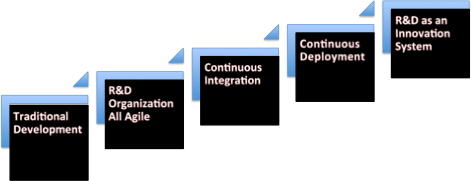
\includegraphics[width=3.5in]{stairway.png}
	\caption{Organization evolution path \cite{olsson2012climbing}.}
\end{figure}

%In this thesis we conduct a case study to analyse the adoption of continuous deployment and continuous experimentation in B2B domain. The case study consists of a literature review on applications of these practices, an interview of key members in the case company and analysis of the results. 

The study is an exploratory deductive case study, which aims to explore how continuous deployment and continuous experimentation can be integrated to the development process. The study specifically aims to identify the main requirements, problems and key success factors with regards to these approaches. Integrating these approaches to the development process requires a deep analysis of the current development process, seeking the current problems and strengths. Adopting both continuous deployment and continuous experimentaton also requires understanding the requirements of continuous deployment and continuous experimentation, and restrictions caused by the developed software product.

In this research, the units under the study are two teams responsible for developing two different software products. By focusing on different products, a broader view on the application of these development approaches can be gained. The other product, a marketing automation called Dialog, is used through an extensive user interface. The other product under inspection, CDM, is a Master Data Management \cite{loshin2010master} solution running as a background application. The objective of this thesis can be therefore summared as follows:

\bigskip
\noindent \textbf{Research objective}
To analyze the software development process transition towards shorter feedback cycle and data-driven decisions from the perspective of the case company, with respect to continuous delivery and continuous experimentation practices.

\subsection{Research questions}

The broader research objective is explored here. \newline
%Literature review / Interview
\noindent \textbf{RQ 1: What are the B2B specific challenges of continuous delivery and continuous experimentation?}

\noindent In B2B domain the connection with end users might not be established properly, and the customer feedback might only be received from certain key members. Running experiments on customer environments also requires a new deployment of the software product. The purpose of this research question is to identify the differences in the software development process and the product in B2B and B2C environments, and it is answered based on both literature review and interview. 
Question: contractual issues? 
Question: selecting the correct OEC in b2b is harder. for example revenue. 
question: in B2C people develop their own product, but in B2B the feature ideas might come only from customer.
\newline

%collect ideas from literature review and interview
%\noindent \textbf{RQ 2: How to collect usage data and customer feedback in B2B domain, where user amounts can be very low?}

%\noindent Research question 4 is answered by analysing the usage data and customer feedback collection of the case company. This is carried out by interviewing the key persons responsible for customer interaction and developers responsible for usage data collection.  

%As compared to the B2C domain where the product is often deployed in cloud with a lot of users, B2B applications might only have a handful of users. This question %is answered by collecting ideas from the literature review and interview results. \newline
%-Legal issues
%-Technical issues

%Interview results have to be compared to literature review results
\noindent \textbf{RQ 2: How do continuous delivery and continuous experimentation benefit the case company?} %What are the problems and strengths of the current development process?

\noindent To rationalize the decision to adopt continuous delivery and experimentation in a company, the actual benefits to the business have to be identified. This question is answered by comparing problems and benefits of literature review to the results of the interview. \newline

One idea is also to aid marketing by selling the MVPs to customers. This way we can pivot the product with customers, they can test it in practice and then decide whether to pay for the product or not. \newline

%\noindent \textbf{RQ 3: What is the Minimum Viable Process of continuous experimentation?}

%\noindent While a definitive process of continuous experimentation hasn't been defined, a process with multiple different roles is quite heavyweight and not quickly adoptable. The purpose of this research question is to identify the core practices and requirements of continuous experimentation. How can the process be kept as simple as possible without losing the benefits? The goal is that companies are able to quickly test whether the process suits their needs. This requires that the process is defined in such level of abstraction that it can be adopted in practice with relative ease. This research question is answered based on literature %review. To answer this research question, a deep understanding of the process has to be established. \newline

%collect ideas from literature review and interview
\noindent \textbf{RQ 3: How can continuous experimentation be systematically organised in the B2B domain?}

\noindent When the benefits and requirements are identified and the process is approved by a company, it has to be adopted in practice. This requires an answer to questions what, how, who and when. This question is answered by applying Fagerholm et al. model \cite{fagerholm2014building} to two different teams and software products within the case company, and addressing the challenges found in the first research question. \newline
%-Where do the feature ideas come from?
%-What roles are required?
-What kind of deviations are there in the model?

\subsection{Scope and limitations}
This study focuses on the 

The background theory is drawn from literature focusing on continuous delivery, continuous experimentation, lean startup and experiment innovation systems. 

The empirical research of this thesis has been carried out in the context of a medium sized information technology company, Steeri Oy. The company specializes in customer data on multiple fronts: CRM, BI, Master Data Management and data integrations, among others. The empirical research has applied case study methodology to offer deep understanding of the phenomena in their natural context. The tradeoff of a case study research is that they do not provide much room for direct generalizations outside the empirical context. 

This thesis is organized as follows. The first chapter is the introduction at hand. The second and third chapter summarize the relevant literature and theories to position the research and to educate the reader on the body of knowledge and where the contributions are intended. The fourth chapter briefly explains the usage of case study and qualitative research as research methods, to provide background for the decision to utilize them in this particular study. The fifth chapter presents the research design: objectives, context and applied methods. The findings are then presented in the sixth chapter. 
%Structure:
%
%#1
%Background information - case study context - results - limitations - summary, future work
%#2
%Related work - experimental setup - results - summary
%-GOAL OF THE THESIS
%-motivation
%-research question
%-approach
%>analyze state of the practice
%>specify problem and goals 
%>analyze state of the art
%>state hypotheses
%>derive solution idea

\section{Literature: Continuous Delivery}
%Agile
Agile software development emerged from the iterative software development methods, with early implementations being development in the 1990's \cite{dybaa2008empirical}. The general principles of agile software development are breaking the development to short iterations, maintaining a short feedback loop with the customer by having a customer representative, valuing working software over documentation and responding to change.

%Agile implementations
Many agile models, such as Scrum \cite{schwaber2002gile}, Extreme Programming \cite{beck2000extreme} and Feature-Driven Development \cite{palmer2001practical} further defined their own strategies based on the agile principles. Scrum, for example, defines a framework for managing product development, without much focus on technical tools. Extreme Programming, on the other hand, includes many technical features, such as always programming in pairs, doing extensive code review and unit testing all code.

%Lean manufacturing & LSD
Lean manufacturing, derived from the Toyota Production System \cite{ono1988toyota}, is a streamlined production philosophy that aims to identify the expenditure of resources not used in creating value for the end customer, and eliminate these activities. Lean software development \cite{poppendieck2003lean} has been developed based on the same idea. The purpose of lean software development is to eliminating waste, or anything that doesn't bring value to the customer, and to pursuit perfection through smoothing the development flow. The principles in lean software development are eliminate waste, amplify learning, decide as late as possible, deliver as fast as possible, engage everyone, build quality in and see the whole. 

%Lean startup
Lean startup \cite{ries2011lean} is a business and product development method with focus on business-hypothesis-driven experimentation and iterative product releases. A primary purpose of lean startup is to assess the specific demands of consumers and to fulfill those demands with the least possible resources. This is achieveved by using a Build-Measure-Learn-loop, which is used to learn the customers actual needs and consecutively to steer business and product strategies to the correct direction. The tight customer feedback loop ensures that the product development doesn't include features and services not wanted by the customer. 

TODO:
-Stairway to heaven
-Innovation experiment system

\subsection{Development pipeline}

\subsection{Continuous deployment}

To be able to react to customers changing requests and manage multiple customer environments, the software product has to be deployed frequently and with different configurations. As the case company is working in an agile manner, requests change and adjust often. To improve the software product, the case company has a need for a deployment approach that has the following benefits.

\begin{itemize}
\item Fast feedback on changes
\item Automation of repetitive actions
\item Validating that deployed code has passed automatised tests 
\item Traceable. large history records and changelogs
\item Configurable per customer environment
\end{itemize}

Fast feedback is used to validate the functionality of the software and to ensure that quality requirements are met. Automation of repetitive actions ensures that the actions are performed exactly as instructed, without room for manual error. Reducing the amount of manual work also improves efficiency. With traceable history records, troubleshooting process can be shortened. With changelogs, the customer can be kept informed of the changes in new versions. A design practice filling the aforementioned benefits is called Continuous deployment.

%what is it
Continuous deployment is an extension to continuous integration, where the software functionality is deployed frequently at customer environment. While continuous integration defines a process where the work is automatically built, tested and frequently integrated to mainline \cite{fowler2006continuous}, often multiple times a day, continuous deployment adds automated acceptance testing and deployment. The purpose of continuous deployment is that as the deployment process is completely automated, it reduces human error, documents required for the build and increases confidence that the build works \cite{cdbook}. 

%release cycles
In an agile process software release is done in periodic intervals \cite{cockburn2002agile}. Compared to waterfall model it introduces multiple releases throughout the development. Continuous deployment, on the other hand, attemps to keep the software ready for release at all times during development process \cite{cdbook}. Instead of stopping the development process and creating a build as in an agile process, the software is continuously deployed to customer environment. This doesn't mean that the development cycles in continuous deployment are shorter, but that the development is done in a way that makes the software always ready for release.
\begin{figure}[h]
	\centering
	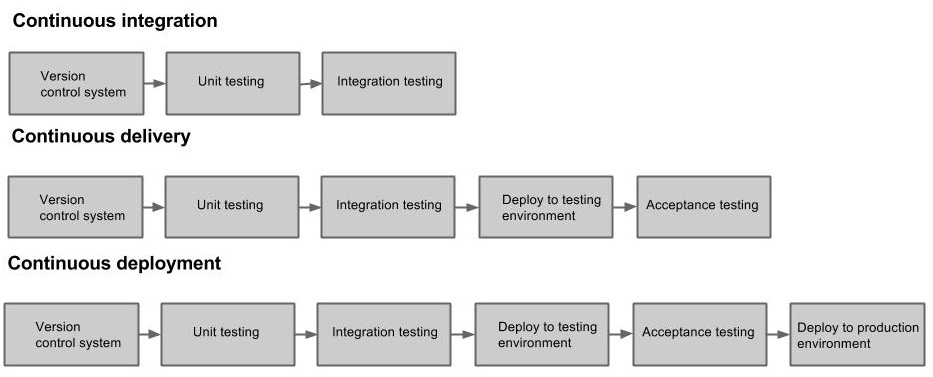
\includegraphics[width=3.5in]{rtvd.jpg}
	\caption{Continuous integration, delivery and deployment.}
	\label{fig1}
\end{figure}
%delivery vs deployment
Continuous delivery differs from continuous deployment. Refer to Fig. \ref{fig1} for a visual representation of differences in continuous integration, delivery and deployment. Both include automated deployment to a staging environment. Continuous deployment includes deployment to a production environment, while in continuous delivery the deployment to a production environment is done manually. The purpose of continuous delivery is to prove that every build is proven deployable \cite{cdbook}. While it necessarily doesn't mean that teams release often, keeping the software in a state where a release can be made instantly is often seen beneficial.

%Barriers in CI->CD transition: stairway
Holmström Olsson et al. have researched the transition phase from continuous integration to continuous delivery, and have identified barriers that companies need to overcome to achieve the transition \cite{olsson2012climbing}. One of such barrier is the custom configuration at customer sites. Maintaining customized solutions and local configurations alonside the standard configurations creates issues. The second barrier is the internal verification loop, that has to be shortened not only to develop features faster but also to deploy fast. Finally, the lack of transparency and getting an overview of the status of development projects is seen as a barrier.

Olsson et al. state that in order to shorten the internal verification loop, different parts in the organization should also be involved, especially the product management as they are the interface to the customer. Olsson et al. also note that finding a pro-active lead customer is also essential to explore and form a new engagement model.

\subsubsection{Deployment pipeline}
An essential part of continuous deployment is the deployment pipeline, which is an automated implementation of an application's build, deploy, test and release process \cite{cdbook}. A deployment pipeline can be loosely defined as a consecutively executed set of validations that a software has to pass such before it can be released. Common components of the deployment pipeline are a version control system and an automated test suite.

Humble and Farley define the deployment pipeline as a set of stages, which cover the path from a committed change to a build \cite{cdbook}. Refer to Fig. \ref{fig2} for a graphical representation of a basic deployment pipeline. The commit stage compiles the build and runs code analysis, while acceptance stage runs an automated test suite that asserts the build works at both functional and nonfunctional level. From there on, builds to different environments can be deployed either automatically or by a push of a button.

Humble et al. define four principles that should be followed when attempting to automate the deployment process \cite{humble2006deployment}. The first principle states that "Each build stage should deliver working software". As software often consists of different modules with dependencies to other modules, a change to a module could trigger builds of the related modules as well. Humble et al. argue that it is better to keep builds separate so that each discrete module could be built individually. The reason is that triggering other builds can be inefficient, and information can be lost in the process. The information loss is due to the fact that connection between the initial build and later builds is lost, or at least causes a lot of unnecessary work spent in tracing the triggering build. 

The second principle states that "Deploy the same artifacts in every environment". This creates a constraint that the configuration files must be kept separate, as different environments often have different configurations. Humble et al. state that a common anti-pattern is to aim for 'ultimate configurability', and instead the simplest configuration system that handles the cases should be implemented.
\begin{figure}[h]
	\centering
	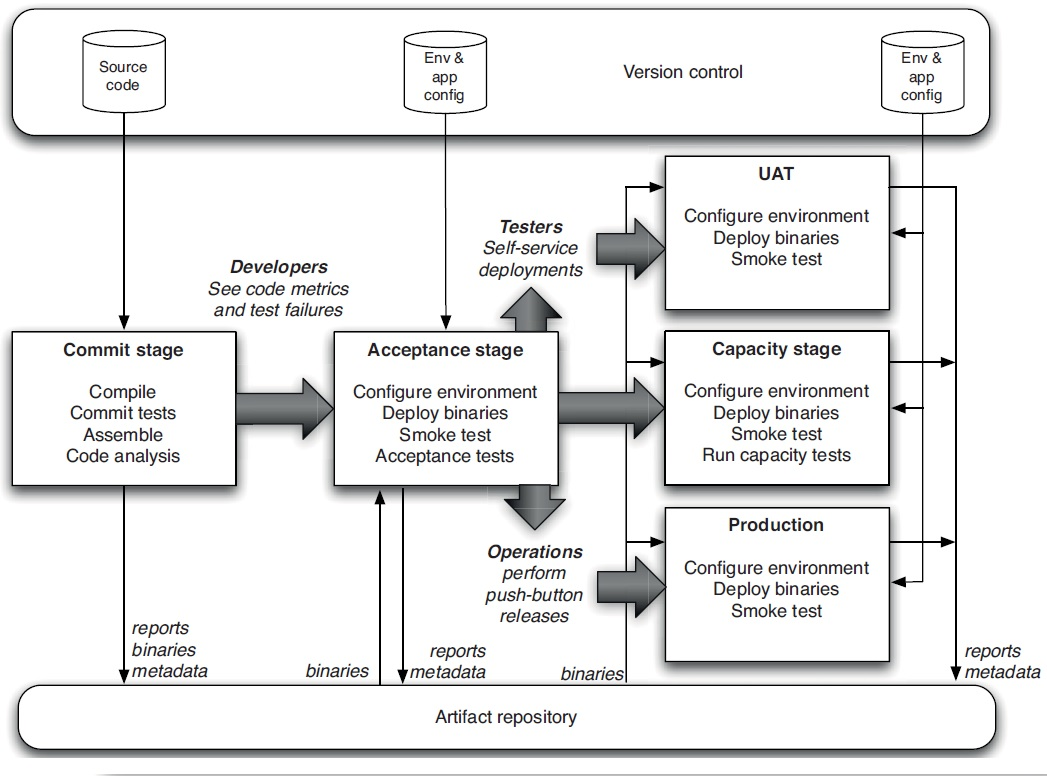
\includegraphics[width=3.5in]{pipeline.jpg}
	\caption{A basic deployment pipeline \cite{cdbook}.}
	\label{fig2}
\end{figure}
Another principle, which is the main element of continuous deployment, is to "Automate testing and deployment". Humble et al. argue that the application testing should be separated out, such that stages are formed out of different types of tests. This means that the process can be aborted if a single stage fails. They also state that all states of deployment should be automated, including deploying binaries, configuring message queues, loading databases and related deployment tasks. Humble et al. mention that it might be necessary to split the application environment into $slices$, where each slice contains a single instance of the application with predetermined set of resources, such as ports and directories. $Slices$ make it possible to replicate an application multiple times in an environment, to keep distinct version running simultaniously. Finally, the environment can be smoke tested to test the environments capabilities and status.

The last principle states "Evolve your production line along with the application it assembles". Humble et al. state that attempting to build a full production line before writing any code doesn't deliver any value, so the production line should be built and modified as the application evolves. 

\subsubsection{Impact on development model}

A picture of the typical development process in continuous deployment is shown in Fig. \ref{fig3}. After the team pushes a change to the version control system, the project is automatically built and tests are triggered stage by stage. If a test stage fails, feedback is given and the deployment process effectively cancelled. In a continuous delivery process, the last stages are approved and activated manually, but in a continuous deployment process the last stages are triggered automatically as well.

\begin{figure}[h]
	\centering
	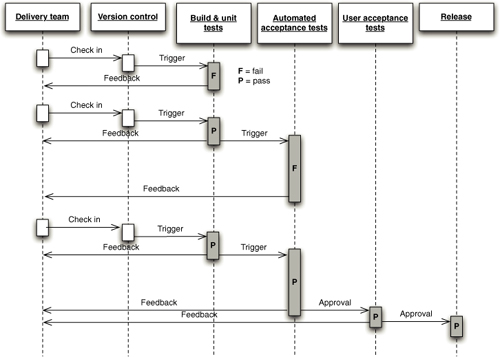
\includegraphics[width=3.5in]{developmentprocess.jpg}
	\caption{Components of the development process \cite{cdbook}.}
	\label{fig3}
\end{figure}


\subsection{Challenges regarding continuous delivery}

"With continuous flow, Sales and Marketing were not quite sure when anything would be released." "We had to provide mechanisms where they could track the status of work in real time, so they can plan accordingly." \cite{neely2013continuous}

-Technical implementation
-Education on the subject
-Active participation of employees

\section{Literature: Continuous Experimentation}

\subsection{Continuous experimentation}
-for a method: what, how, when, who

%Continuous experimentation term
Continuous experimentation is a term created by Dane McKinley, a Principal Engineer at Etsy \cite{mcfunley}. McKinley defines the key aspects of continuous experimentation as making small, measurable changes, staying honest and preventing the developers from breaking things. With staying honest, McKinley implies that the product releases are tracked and measured, so that it's possible to tell whether things went worse or better. McKinley also states that design and product process must change to accomodate experimentation, and that experimenting should be done with minimal version of the idea. When experimentations are implemented and measured, counterintuitive results will be found, and planning to be wrong should be considered \cite{mcfunley}. 
%Prefer incremental redesigns. 

%Continuous experimentation intro
While continuous experimentation is only loosely defined by McKinley, it poses resemblance to multiple development models. One of such models is the Innovation Experiment System \cite{bosch2012building}. The key principles in these development models are data-driven decisions, linking product development and business aspect, reacting to customers present needs, turning hypotheses into facts, failing fast and steering the development process. Fagerholm et al. define that a suitable experimentation system must be able to release minimum viable products or features with suitable instrumentation for data collection, design and manage experiment plans, link experiment results with a product roadmap and manage a flexible business strategy \cite{fagerholm2014building}. The Build-Measure-Loop of Lean Startup is similar in the sense that controlled experiments drive the development.

%Lean startup
In Lean startup methodology \cite{ries2011lean} experiments consist of Build-Measure-Learn cycles, and are tightly connected to visions and the business strategy. The purpose of a Build-Measure-Learn cycle is to turn ideas into products, measure how customers respond to the product and then to either pivot or persevere the chosen strategy. The cycle starts with forming a hypothesis and building a minimum viable product (MVP) with tools for data collection. Once the MVP has been created, the data is analyzed and measured in order to validate the hypothesis. To persevere with a chosen strategy means that the experiment proved the hypothesis correct, and the full product or feature can is implemented. However, if the experiment proved the hypothesis wrong, the strategy is changed based on the implications of a false hypothesis.

%Evolution path
Holmström Olsson et al. have researched the typical evolution path of companies \cite{olsson2012climbing}. The final stage of the evolution phase is when development is driven by the real-time customer usage of software. Defined as "R\&D as an 'experiment system'", the entire R\&D system acts based on real-time customer feedback and development is seen as addressing to customers present needs. At the same time deployment of software is seen as a "starting point for 'tuning' of functionality rather than delivery of the final product". While the evolution from continuous deployment to innovation system wasn't explored, Olsson et al. anticipate that the key actions required are the automatical data collection components and capability to effectively use the collected data.

TODO: Maybe something about continuous innovation? Brown, 1997, The art of continuous change: Linking complexity theory and time-paced evolution in relentlessly shifting organizations

-Connect CE, IES, Microsoft stuff, Lean startup stuff

%In the context of this thesis, Continuous Experimentation refers to a development model following these principles: TODO: improve this
%\begin{itemize}
%\item  \textbf{Data driven decisions}
%\item  \textbf{Link product development and business aspect}
%\item  \textbf{Reacting to customers present needs}
%\item  \textbf{Turning hypotheses into facts}
%\item  \textbf{Steering development process}
%\end{itemize}

"A detailed framework for conducting systematic, experiment-based software development has not been elaborated" \cite{fagerholm2014building}.

A model of continuous experimentation has been created by Fagerholm et al. \cite{fagerholm2014building}. 

%Experiment
An experiment is essentially a procedure to confirm the validity of a hypothesis. In software engineering context, experiments attempt to answer questions such as which features are necessary for a product to succeed, what should be done next and which customer opinions should be listened to. According to Jan Bosch, "The faster the organization learns about the customer and the real world operation of the system, the more value it will provide" \cite{bosch2012building}. Most organizations have many ideas, but the return-on-investment for many may be unclear and the evaluation itself may be expensive \cite{kohavi2007practical}. 

%Continuous deployment - continuous experimentation integration
Continuous deployment attempts to deliver an idea to users as fast as possible. Continuous experimentation instead attempts to validate that it is, in fact, a good idea. In continuous experimentation the organisation runs controlled experiments to guide the R\&D process. The development cycle in continuous experimentation resembles the build-measure-learn cycle of lean startup. The process in continuous experimentation is to first form a hypothesis based on a business goals and customer "pains" \cite{bosch2012building}. After the hypothesis has been formed, quantitative metrics to measure the hypothesis must be decided. After this a minimum viable product can be developed and deployed, while collecting the required data. Finally, the data is analyzed to attempt to validate the hypothesis.

%innovation experiment system
Jan Bosch has widely studied continuous experimentation, or innovation experiment systems, as a basis for development. The primary issue he found is that "experimentation in online software is often limited to optimizing narrow aspects of the front-end of the website through A/B testing and inconnected, software-intensive systems experimentation, if applied at all, is ad-hoc and not systematically applied" \cite{bosch2012building}. The author realized that for different development stages, different techniques to implement experiments and collect customer feedback exist. Bosch also introduces a case study in which a company, Intuit, adopted continuous experimentation and has increased both the performance of the product and customer satisfaction.

\cite{eklund2012architecture}
Applied the continuous experimentation research to embedded software.
"Improvement occurs in individual software parts, but the underlying design concept remain mostly unchanged [3]"
"The experiment infrastructure allows developers to deploy new software and collect data how it behaves in areal-world settings being used by actual users. The infrastructure support deployment of software experiments and collection of data over-the-air on a scale comparable to the entire customer base". 
"The infrastructure supports with automated randomisation and factorial designs [6] sufficient to draw statistical conclusions from the experimental scenarios."
"The experiment manager architecture, seen in Figure 3, supports the deployment of multiple experimental software parts to the same device and autonomously controls when to run which experiment, even allowing for local A/B-testing. Measurements and analysis is done on-board in real-time. The experiment scenario to be answered is implemented on the embedded device (i.e. how long does it take to . . . )"
TODO: picture here

\subsubsection{Experimentation planning}

\subsubsection{Experimentation stages and scopes}
Fig. \ref{fig4} introduces different stages and scopes for experimentation. For each stage and scope combination, an example technique to collect product performance data is shown. As startups often start new products and older companies instead develop new features, experiments must be applied in the correct context. Bosch states that for a new product deployment, putting a minimal viable product as rapidly as possible in the hands of customers is essential \cite{bosch2012building}. After the customers can use the product, it is often not yet monetizable but is still of value to the customer. Finally, the product is commercially deployed and collecting feedback is required to direct R\&D investments to most valuable features.
\begin{figure}[h]
	\centering
	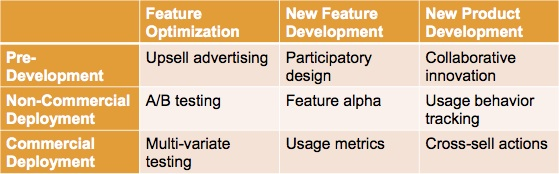
\includegraphics[width=3.5in]{scopes.jpg}
	\caption{Scopes for experimentation \cite{bosch2012building}.}
	\label{fig4}
\end{figure}

\subsubsection{Components in continuous experimentation}
Kohavi et al. investigate the practical implementations of controlled experiments on the web \cite{kohavi2007practical}, and state that the implementation of an experiment involves two components. The first component is a randomization algorithm, which is used to map users to different variants of the product in question. The second component is an assignment method which, based on the output of the randomization algorithm, determines the contents that each user are shown. The observations then need to be collected, aggregated and analyzed to validate a hypothesis. Kohavi et al. also state that most existing data collection systems are not designed for the statistical analyses that are required to correctly analyze the results of a controlled experiment.

The components introduced by Kohavi et al. are aimed primarily for A/B testing on websites. Three ways to implement the assignment methods are shown. The first one is traffic splitting, which directs users to different fleet of servers. An alternative methods is server-side selection, in which API calls invoke the randomization algorithm and branch the logic based on the return value. Last alternative is a client-side selection, in which the front-end system dynamically modifies the page to change the contents. Kohavi et al. state that the client-side selection is easier to implement, but it severely limits the features that may be subject to experimentation. Experiments on back-end are nearly impossible to implement in such manner.

\subsubsection{Data collection}
"Active customer feedback is concerned with surveys and other mechanisms where the customer is aware that he or she is providing feedback. Passive feedback and usage data is collected while the customer is using the system. Examples include the amount of time a user spends using a feature, the relative frequency of feature selections, the path that the user takes through the product functionality, etc. The low cost and ease of data collection leads to the next major difference between IES-based and traditional software." \cite{bosch2012building}

To collect, aggregate and analyze the observations, raw data has to be recorded. According to Kohavi et al., some raw data could be for example page views, clicks, revenue, render time and customer-feedback selections \cite{kohavi2007practical}. The data should also be annotated to an identifier, such that conclusions can be made from it. Kohavi et al. present three different ways for collecting raw data. The first solution is to simply use an existing data collection tool, such as Webmetrics. However, most data collection systems aren't designed for statistical analyses, and the data might have to be manually extracted to an analysis environment. A different approach is local data collection, in which a website records data in a local database or log files. The problem with local data collection is that each additional source of data, such as the back-end, increases the complexity of the data recording infrastructure. The last model is a service-based collection, in which service calls to a logging service are placed in multiple places. This centralizes all observation data, and makes it easy to combine both back-end and front-end logging.  

\subsubsection{Data analysis}
To analyze the raw data, it must first be converted into metrics which can then be compared between the variants in a given experiment. An arbitrary amount of statistical tests can then be run on the data with analytics tools in order to determine statistical significance. 

\subsubsection{Roles in continuous experimentation}
Fagerholm et al. define five different roles in continuous experimentation: Business Analyst, Product Owner, Data Analyst, Software Developer and Quality Assurance \cite{fagerholm2014building}. The business analyst along with the product owner are responsible for creating and updating the strategic roadmap, which is the basis of the hypotheses. The basis for decisions are the existing experimental plans and results stored in a database. A data analyst is used to analyze the existing experiments and results and to create assumptions from the roadmap. The analyst is also responsible for the design and execution of experiments. The data analyst is in tight collaboration with the software developer and quality assurance, who are reponsible for the development of MVPs and MVFs. The software designers create the necessary instrumentations used to collect the data required by the analyst.


TODO: adobe:
Pipeline team: designer, developer, researcher, product manager \cite{adobe}

%question: what if there are no existing experimental plans, and this is the first experiment? how should the roadmap be created?

\begin{figure}[h]
	\centering
	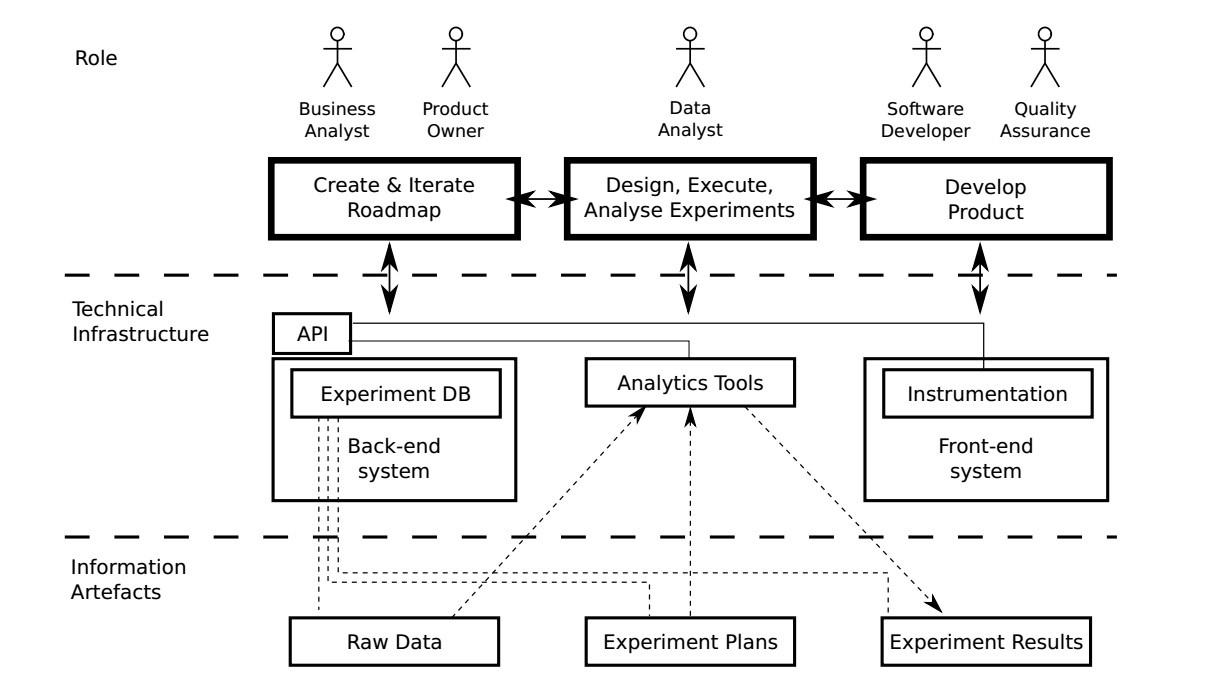
\includegraphics[width=5in]{infra.jpg}
	\caption{Continuous experimentation infrastructure \cite{fagerholm2014building}.}
	\label{fig4}
\end{figure}

%http://www.janbosch.com/Jan_Bosch/Innovation_Experiment_Systems.html
\subsection{Continuous deployment and continuous experimentation collaboration}
As the experiments are run in a regular fashion, integrating experiments to the deployment pipeline should be considered. This requires changing the development process in such fashion that functionality is developed based on some actual data. The components required to support continuous experimentation include tools to assign users to treatment and control groups, tools for data logging and storing, and analytics tool for conducting statistical analyses.

\subsection{Challenges regarding continuous experimentation}
"Experimentation in practice is often limited to optimizing narrow aspecs of the front-end through A/B testing, and is not systematically applied" \cite{bosch2012building} 

"Collecting customer or performance data early in the innovation process requires changes to the R\&D processes, as customers need to be involved much earlier and deeper in the process. This also requires architectural changes of the product and platform to determine customer preference and interest." \cite{bosch2012building}

"A final aspect is the avoidance of versioning of software. Traditionally, for many companies, every customer would ultimately have a unique configuration of the product with different versions of components making up the system. This adds a whole new layer of complexity to the already costly process of deploying new versions. In an IES environment, there is only one version: the currently deployed one. All other versions have been retired and play no role." \cite{bosch2012building}

"Innovation in large organization is often characterized by an enormous imbalance between the number of ideas that, informally or formally, exist in the organization and the number of concepts that are in fact tested with customers." \cite{bosch2012building}

"Traditional metrics such as the Net Promoter Score[Reichheld, F.F.: The One Number You Need to Grow] have been used for the last decade or more, but often fail to provide timely feedback during the development process as these are backward looking and focus on the entire product." \cite{bosch2012building}

"Most organizations have many ideas, but the return-on-investment (ROI) for many may be unclear and the evaluation itself may be expensive." \cite{kohavi2007practical}

TODO: possible challenges in Lean Startup: \cite{may2012applying}

-Randomization algorithm and assignment method, data collection, storage, analysis \cite{kohavi2007practical}

Pitfalls:
\begin{center}
\begin{table}[htb]
    \begin{tabular}{ | p{2cm} | p{10cm} |}
    \hline
	Pitfall 1 & Picking an OEC for which it is easy to beat the control by doing something clearly “wrong” from a business perspective \\ \hline
	Pitfall 2 & Incorrectly computing confidence intervals for percent change and for OECs that involve a nonlinear combination of metrics \\ \hline
	Pitfall 3 & Using standard statistical formulas for computations of variance and power \\ \hline
	Pitfall 4 & Combining metrics over periods where the proportions assigned to Control and Treatment vary, or over subpopulations sampled at different rates \\ \hline
	Pitfall 5 & Neglecting to filter robots \\ \hline
	Pitfall 6 & Failing to validate each step of the analysis pipeline and the OEC components \\ \hline
	Pitfall 7 & Forgetting to control for all differences, and assuming that humans can keep the variants in sync \\ \hline
    \end{tabular}
    \caption{Pitfalls to avoid when running controlled experiments on the web \cite{crook2009seven}.}
    \end{table}
\end{center}

-Roles
-Environment
-Deployment

\subsection{(TODO:move\&rename)Why is this interesting?}
%However, based on the state-of-the practice section (describing 
%what is currently done in industry) you should motivate that the 
%problem you are addressing is a significant problem in industry 
%(you can include this justification at the end of the section).
%Why is this interesting?

"Companies are increasingly transitioning their traditional research and product development functions towards continuous experiment systems" \cite{olsson2012climbing}. TODO check this

"The literature is increasingly recognizing the importance of continuous innovation" \cite{steiber2013corporate}

\subsection{(TODO:move\&rename)Existing case studies}
%At the end of the state-of-the-art section you should describe the differences
%between existing related research approaches (and especially existing 
%case studies) and compare them with your own goal in order to motivate your
%study.

%Previous works have presented case studies that exhibit di↵erent
%aspects concerning continuous experimentation. Steiber [23] report
%on a study of the model of continuous experimentation followedby Google, analysing a success story of this approach. Adams [1]
%present a case study on the implementation of Adobe’s Pipeline, a
%process that is based on the continuous experimentation approach.

Existing case studies regarding continuous experimentation have been conducted with varying aspects under concentration. Olsson et al. conducted a multiple-case study to explore companies moving towards continuous deployment and continuous experimentation \cite{olsson2012climbing}. In the transition phase from continuous integration stage to continuous deployment, the study investigates a telecommunications company with a highly distributed organization. The study considers transition from continuous delivery to continuous experimentation as a future research interest. 

Case study: stairway to heaven \cite{olsson2012climbing}
  -multiple-case study exploring companies moving towards continuous deployment 
  -evolution phases, no continous experimentation transition defined
  -Continuous delivery transition with a highly distributed team
  -R\&D as an experiment system

Fagerholm et al. analytically derive a continuous experimentation model and apply it in practice in a startup company \cite{fagerholm2014building}. The study introduces an initial continuous experimentation model, 

Case study: building blocks \cite{fagerholm2014building}
  -analysis of a continuous experimentation model in the case company
  -design science research that derives a model and applies it in practice
  -initial continuous experimentation model
  -startup company 

Case study \cite{steiber2013corporate}
  -continuous innovation "an experimental iterative process that operates successively to solve problems in markets characterized by turbulence, uncertainty and complex interactions"
  -continuous innovation, "the ability to renew the organization and to develop new products and business models, is central for most companies"
  -specifies in organizational characteristics
  -innovational culture aspects
  -Steiber [23] report on a study of the model of continuous experimentation followed by Google, analysing a success story of this approach.

Case study \cite{adams2013creating, adobe}
  - Adams [1] present a case study on the implementation of Adobe’s Pipeline, a process that is based on the continuous experimentation approach.
  - Innovation pipeline:
  1 collect user problems
  2 ID problems worth solving
  3 prototype possible solutions
  4 live user testing + public releases
  5 refine, pivot or kill the idea
  6 build products that understand the user

  Pipeline team: designer, developer, researcher, product manager

  General principles: 
  the idea will change
  we're only right when the market tells us so
  create fast. improve constantly
  find the simplest thing that could possibly work
  define "success" before we build
  fail forward
     -accept failure as part of our process not the end of it 
     -fail often, but make mistakes on a small scale
     -always learn from what went wrong
     -don't fall in love. remain open to the pivot
     -don't let them ruin good with perfect

(Case: online experimentation at microsoft \cite{kohavi2009online})

Motivation: %Compare to my own goals
  -clearly defined in the B2B context
  -

\section{Case study as a research method}

\subsection{Case study}
Case study is a way to collect data through observation and to test theories in an unmodified setting \cite{zelkowitz1998experimental}. The case in a case study is the situation, individual, group or organization that the researchers are interested in \cite{robson2002real}. Kitchenham et al. found case studies important for industrial evaluation of software engineering methods and tools \cite{kitchenham1995case}. Runeson and Höst define it as a suitable research method for software engineering, since it studies contemporary phenomena in its natural context \cite{runeson2009guidelines}. It might not be possible to generate causal relationships from case studies as compared to controlled experiments. However, they provide a deeper understanding of the unit under study \cite{runeson2009guidelines}. An opposite type of research would be a formal experiment, with a narrow focus and control on variables. 

Case studies can serve different purposes. Robson defines four purposes as Exploratory, Descriptive, Explanatory and Improving \cite{robson2002real}. In an exploratory case study, the purpose is to seek new insights, find out what is happening and generate ideas and hypotheses for new research. Descriptive case study attempts to portray a situation or a phenomenom. Explanatory case study attempts to seek and explanation to a problem or situation, mostly in a causal relationship. An improving case study tries to improve an aspect of the studied phenomenom.  

%http://2012books.lardbucket.org/books/sociological-inquiry-principles-qualitative-and-quantitative-methods/s05-03-inductive-or-deductive-two-dif.html
Different approaches to the order of data collection, analysis and generalization can be categorized into inductive, deductive and abductive approaches \cite{dubois2002systematic}. In an inductive case study the research is conducted by first collecting the data, then looking for patterns and forming theorie that explain those patterns. Therefore an inductive approach moves from data to theory. A deductive approach, on the other hand, is in reversed order; the approach moves from general level to a more specific level. A deductive approach begins with studying what others have done, and then testing hypotheses that emerge from those teories. An abductive approach starts with the consideration of facts, or particular observations. These observations are then used to form hypotheses that relate them to a fact or a rule that accounts for them. The facts are therefore correlated into a more general description, that relates them to a wider context.

Runeson and Höst define the case study structure in five steps \cite{runeson2009guidelines}. First the case study is designed: objectives are defined and the study is planned. Then procedures and protocols for data collection are defined. Then the evidence is collected by executing the data collection on the studied case. The collected data is then analysed, and finally the results are reported.

Triangulation is a way to increase the reliability and validity of the findings. Triangulation means using different data collection methods or angles, and providing a wider picture of the case. Triangulation is especially important for qualitative data, but can also be used for quantitative data to compensate for measurement or modeling errors \cite{runeson2009guidelines}. Stake defines four ways to apply triangulation: Data triangulation, Observer triangulation, Methodological triangulation and Theory triangulation \cite{stake1995art}. In data triangulation, multiple data sources are used, or the data is collected at different occasions. In observer triangulation more than one observer is used in the study. In methodological triangulation different types of data collection methods are combined, such as qualitative and quantitative methods. In theory triangulation alternative theories or viewpoints are used.

Data collection in case studies tend to lean towards qualitative data that provides a richer and deeper view as compared to quantitative data \cite{runeson2009guidelines}. As a data collection method, semi-structured interviews are common in case studies \cite{runeson2009guidelines}. However, generalizing the results of a case study is often a subject of internal validity \cite{kitchenham2002preliminary}. It is especially important in a case study to address reliability and validity of the findings. Even with good faith and intention, biased and selective accounts can emerge \cite{robson2002real}. 

\subsection{Qualitative research}
Qualitative research attempts to answer to questions "Why?"" and "How?" instead of "What?", "Where?" and "When?" as compared to quantitative research. The most common way to collect qualitative data is via an interview. Seaman defines interviews as a way to collect historical data, opinions and impressions about something \cite{seaman1999qualitative}. The interview can be either structured, unstructured or semi-structured. In a structured interview the interviewer asks all of the questions, and the objectives are very specificed. The focus of a structured interview is to find relations between constructs, and the objective is descriptive and explanatory \cite{runeson2009guidelines}. In an unstructured interview the topic is broadly defined, and questions are asked also by the interviewee. In an unstructured interview open-ended questions are typical, and unforeseen types of information can be gained. The focus of an unstructured interview is on how the interviewee qualitatively experience the phenomenom, and the objective is exploratory \cite{runeson2009guidelines}. A semi-structure interview is a mixture of both open-ended and specific questions. Semi-structured interviews focus on how individuals qualitatively and quantitatively experience a phenomenom, and the objective is both descriptive and explanatory \cite{runeson2009guidelines}.

Qualitative data analysis \cite{robson2002real}

Seaman has explored qualitative research in software engineering context, and he defines different ways to analyse qualitative data. \cite{seaman1999qualitative} 
-Coding, extracting values for quantitative variables from qualitative data
-Coding subjective data, select reference points for views, evaluate relability
-Generation of Theory (GoT), extract from a set of field notes a statement or proposition supported in multiple ways by the data - – for use as hypotheses
-GoT cross-case analysis: data divided into “cases”: two groups based on some attribute and examine similarities and differences (devs / management?)
-Confirmation of Theory: target: building up “weight of evidence"; triangulation; anomalies in the data
-qualitative data is richer than quantitative data. use of qualitative methods increases
– amount of information
– diversity of information
– confidence in results

The basic objective of data analysis is to form conclusions and theories from the data based on a chain of evidence. Qualitative data analysis can be divided into two different parts, hypothesis generating techniques and hypothesis confirmation techniques \cite{runeson2009guidelines}. Both of these techniques can be exploratory and explanatory case studies \cite{runeson2009guidelines}.  

%Quasi-statistical approaches, Template approaches, Editing approaches, Immersion approaches 
Robson introduces common features of qualitative data analysis in a sequential list \cite{robson2002real}. The first step is to code the initial set of data. Then, comments and reflections (referred to as 'memos') are added. After this the data is processed, similar phrases, patterns, themes, relationships and differences between sub-groups are identified. These identified patterns are then used to focus the next data collection phase. Gradually a set of generalizations are formed, that cover the consistencies discerned in the data. These generalizations are then linked to a formalized body of knowledge in the form of constructs or theories. 

In the sequential list, hypotheses are identified after the data has been coded. The hypotheses are then used to guide the following data collection process in an iterative approach. During the iterations, some generalizations can be formed, which eventually form a formalized body of knowledge as a final result.

Hypothesis generating techniques are for example "constant comparison method" and "cross-case analysis" \cite{seaman1999qualitative}. In the constant-comparison method the field notes are coded, text pieces are grouped into patterns and propositions that are strongly supported by the data are made. The propositions are then validated against any new data. In the cross-case analysis method data is divided into cases, such as two groups based on the same attribute. Pairs of cases are then compared to determine validations and similarities. 

The data analysis can be conducted with multiple different approaches, with each having a varying degree of formalism. Robson lists four such approaches, from least formal to most formal: Immersion approaches, Editing approaches, Template approaches and Quasi-statistical approaches \cite{robson2002real}. Immersion approaches are the least format, relying mostly on the interpretive skills of the researcher and having a low level of structure. Editing approaches include the usage of some codes which the researcher decides based on findings during the analysis. Template approaches, also known as template analysis, use priori codes to develop a coding template, organising the data based on themes. Quasi-statistical approach is the most formal approach, including quantitative calculations, such as word frequencies. Runeson and Höst state that editing approaches and template approaches are most suitable for software engineering case studies, as a clear chain of evidence is hard to obtain in immersion approaches, and word frequencies are hard to interpret \cite{runeson2009guidelines}. 

\subsubsection{Template analysis}

Template analysis doesn't describe a clearly defined method, but rather refers to a related group of techniques used to thematically organise and analyse textual data \cite{king2004using}. Template analysis is a relatively structured process to analyse textual data, and has mostly been used to analyse data from individual interviews \cite{king2012doing}. The key component in template analysis is the generation of a coding template, which is initially formed on the basis of a subset of the data and then applied to further data. 

King defines code as a label attached to a section of text to index it as a relating to a theme or issue in the data \cite{king2004using}. As an example, codes can be defined to identify points in the text where an interviewee mentions particular categories of presenting problems. These kind of codes can be descriptive, and require no further analysis by the researcher. However, also codes requiring more interpretation can be defined. In template analysis, a key feature is to form a hierarchical organization of codes \cite{king2004using}. This way groups of similar codes are clustered together to form higher-order codes. This way the researcher can analyse the data at different levels of specifity, with higher-order codes giving a broad view and lower-order codes a more specific view. Parallel coding, where the same text segment is categorised with two different codes, is also allowed. 

The process of template analysis is to first create an initial template based on some pre-defined codes \cite{king2004using}. Then the template is revised by working through the data systematically while identifying and coding sections of interest in the text. Based on these findings, the initial template is modified, and finally develops to its final form. Modifications can be either insertion, deletion, changing scope or changing higher-order classification \cite{king2004using}. The final template is such that no sections of text related to research questions remains uncoded. 

The template is then used in interpretation to provide an account. King lists various guidelines that can be used in the interpretation of coded data \cite{king2004using}. The first guideline is to compile a list of all codes with some indication of frequency. The distribution of codes can then help to draw attention to the aspects of data with either multiple codes or missing codes. For example, if one interview in a set of interviews is missing a certain theme, analysis for possible reasons behind that missing code can be made. However, King suggests that while patterns can be used to draw attention to certain parts of the textual data, frequencies alone cannot be to gain any meaningful information. 

Another guideline is selectivity. King states that every code cannot be interpreted to equal degree of depth, and themes most relevant to understanding the phenomena under study must be identified. Prior assumptions of the researched shouldn't limit the analysis. Yet another guideline is openness, which King describes as taking themes judged as marginal into account. Themes that aren't of direct relevance to the initial research questions shouldn't be disregarded, as they can play a useful role in adding to the background of the study. Also themes lying outside the scope of the study should be included in the analysis, if they're considered to cast light on the interpretation of central themes in the study. Finally, King explains that purely linear relationships between codes, such as hierarchical relationships with subsidiary codes next to parent codes, "may not reflect the kinds of relationships a researcher may want to depict in his or her analysis". Instead, maps, matrices and other diagrams can be used to explore and display findings, and analysis doesn't have to stop when a full linear template is produced.

Finally, an account of the interpreted data has to be presented. As with interpretation, King provides three common approaches to presentation \cite{king2004using}. First of the approaches is a set of individual case studies, followed by discussion of differences and similarities between cases. This approach gives a lot of perspective of individuals, but can be confusing if the amount of participants is large. The second approach is an account structured around the main themes identified, drawing illustrative examples from each transcript as required. King states that this is the approach that most readily provides a clear thematic discussion, but the dangers is in drifting towards generalizations and losing sights of individual experiences. The third approach is a thematic presentation of the findings, using a different individual case-study to illustrate each of the main themes. The main problem here lies in selecting the cases which represent the themes in the data as a whole. King also adds that no matter which approach is used, direct quotes from participants is essential.  
%Template TODO: http://www.hud.ac.uk/hhs/research/template-analysis/what-is-template-analysis/ 

\section{Research design}

Research design depicts the strategic decisions that guide how research is carried out \cite{denzin2000discipline}. This includes the studied phenomena, method selection, data-gathering and analysis. Different perspectives towards the researched subjects are usually categorized into two paradigms: positivist and constructivist \cite{gephart2004qualitative}. Positivism contents that an objective reality, which can be studied, captured and understood, exists. Postpositivism argues that reality can never be fully apprehended, but only approximated. Postpositivism therefore relies on multiple methods to capture as much of reality as possible. Constructivism assumes that multiple realities exist. A critical paradigm lies somewhere between positivism and constructivism, assuming that our ability to know of this reality is imperfect. To understand as much of reality as possible, it must be subject to wide critical examination. 

This thesis is based on the critical realist perspective. Critical realism studies people's perceptions to gain understanding of the reality that exists beyond these perceptions \cite{healy2000comprehensive}. Critical realism is especially suitable for case study research if the process involves thoughtful in depth research with the object of understanding why things are as they are \cite{easton2010critical}. 

TODO: triangulation? 

The logical starting point of this thesis was 

\subsection{Objective} %what to achieve?
%What does the company want to achieve
%What are the biggest problems
The purpose of this study is to seek ways to improve the product development process of two products within the case company, using practices known as continuous delivery and continuous experimentation. Existing documented applications of continuous experimentation are primarily executed in the B2C domain, often with a SaaS product. Examples are the Microsoft EXP platform \cite{ep} and Etsy \cite{}. The focus of this study is in the B2B domain, with two applications that are not used as SaaS. 
%As the development process greatly varies in other teams inside the company, the focus is on a single team to narrow the scope.

The study is an exploratory deductive case study, which aims to explore how continuous deployment and continuous experimentation can be integrated to the development process. The study specifically aims to identify the main requirements, problems and key success factors with regards to these approaches. Integrating these approaches to the development process requires a deep analysis of the current development process, seeking the current problems and strengths. Adopting both continuous deployment and continuous experimentaton also requires understanding the requirements of continuous deployment and continuous experimentation. To narrow the scope of the thesis, the focus of this thesis is in the development process of two different software products. The two different products were chosen so that cross-case analysis and therefore more generalizations can be made.

The research design starts by reviewing literature on both continuous delivery and continuous experimentation. In the literature review, main goals are to identify existing requirements and success factors in these approaches. Then interview is used to analyze and identify the pain points the company currently has in its development process. Then continuous deployment and continuous experimentation processes are viewed from the viewpoint of the case company, and possible pains identified. As a result, necessary restrictions and requirements encountered in the B2B domain are obtained. 

The research questions and research methods are summarize in Table 2.

\begin{center}
\begin{table}[htb]
    \begin{tabular}{ | l | p{5cm} | l | p{3cm} |}
    \hline
    Knowledge gap & Research question & The focus of analysis & Data \\ \hline
    a & RQ 1: What are the B2B specific challenges of continuous delivery and continuous experimentation? & Empirical case supported by conceptual analysis & 13 interviews, documentations of the development process, literature \\ \hline
    %a & RQ 2: How to collect usage data and customer feedback in B2B domain, where user amounts can be very low? & Empirical case & 13 interviews, documentations of the development process, literature \\ \hline
    a & RQ 2: How does continuous experimentation benefit the case company? & Empirical case supported by conceptual analysis & 13 interviews, documentations of the development process, literature \\ \hline
    %a & RQ 3: What is the Minimum Viable Process of continuous experimentation? & Conceptual analysis & Literature \\ \hline %How can the process be simplified without losing the benefits?
    a & RQ 3: How can continuous experimentation be systematically organised in the B2B domain & Empirical case supported by conceptual analysis & 13 interviews, documentations of the development process, literature \\ \hline
    \end{tabular}
    \caption{Research questions and research methods.}
    \end{table}
\end{center}

In this thesis along with confirming existing theories we do aim to generate new concepts and theories. The theory and case analysis are continuously matched to gain insights coherent with both theory and empirical observations. 

\subsection{Case descriptions} %what is studied?
%Be sure to specify as much of the industrial context as possible. In particular,
%clearly define the entities, attributes, and measures that are capturing the contextual information.

Experimental context needs the three elements: background information, discussion of research hypotheses, and information about related research \cite{kitchenham2002preliminary}. The two former will be discussed here, and the latter in the section "Frame of reference".

-configuration management: no employer designed and no formal education

The company in question is Steeri Oy, which is a medium-sized company specializing in managing, analyzing and improving the usage of customer data. In this research, the units under the study are two teams responsible for developing two different software products. The first team is the Development \& Integration, which is further split into two sub-teams: Dialog and CDM. Both of the subteams develop a different product. The team is managed by a Concepting \& Management team, which consists of the Product Owners of both software products, quality assurance and commercialisation experts. 

The organisation of Steeri Oy is of a divisional type, with each business area forming independent teams based on the products and projects. The subteams of the first team under study have a common team leader, but different product owners and middle management. TODO: describe organisation structure %: https://docs.google.com/a/steeri.fi/spreadsheet/ccc?key=0Ai02aScOCplAdG9zQURicnlkM0ptTXhqbHN5ZE04X0E&usp=drive_web#gid=0

The unit of analysis is the development process of the two teams. The whole development process consists of the development framework used, but also of the interaction with customers, tools used in the current development process and the roles of individuals in the process. The unit of analysis is studied by focusing on interviewing individual members at different positions in the organisation. The purpose of the interview is to identify the pain points in the development process regarding continuous deployment and continuous experimentation. 

Continuous deployment and continuous experimentation haven't been previously used by the case company. 

In the beginning of the study, feedback was only collected in the form of bug reports from the customers. The bugs were then prioritized according to the importance, and added into the Trello workflow. 

Under analysis is also the company's ways to interact with the customer.

The development process of the team is elaborated in detail in the chapter "State of the practice". In the following sections the general characteristicts of the two products and development processes used are identified and compared. The general characteristics are as follows. 

\begin{multicols}{2}
\begin{itemize}
  \item Product description
  \item Product environment
  \item Product architecture
  \item Users of the software component
  \item Team composition
  \item Development practice
  \item Business model TODO: validate if this is confidental
  \item Programming languages
  \item Development tools
  \item Version releasing
  \item Unit testing
  \item Acceptance testing
  \item Feedback collection
  \item Usage data collection
  \item Feedback and usage data usage
\end{itemize}
\end{multicols}

The first three characteristics give us information on how the teams develop their software products. Testing is used to.. TODO: explain the general characteristics

\subsubsection{Dialog}
The Dialog subteam focuses on developing a multi-channel online marketing automation, iSteer Dialog. It is a software product designed to allow effective marketing on multiple channels, such as e-mail and websites, and to automate repetitive tasks. The product can be integrated to existing CRM solutions, and the data stored in CRM can then be effectively used for marketing purposes. 

\begin{description}
  \item[Product description.] Dialog is a multi-channel online marketing automation tool. The purpose of the product is to allow effective marketing on channels such as e-mail and websites, and to automate repetitive tasks. The product can be integrated to existing CRM solutions, and the data stored in the CRM can then be effectively used for marketing purposes. The product is primarily used through a comprehensive user interface by marketing professionals of customer companies. 
  \item[Product environment.] The product can be run on either servers provided by the case company or on the customers internal servers. Most of the customers use the product on the case companys own servers. Each customer using a provided server has an individual server and configurations, due to different integrations to the customers own systems. Customers running the product on their own servers form a minority.
  \item[Product architecture.] The product consists of a single maven-packaged project. Along with the actual product, several additional third-party or custom components are required. Such components are for example Typo3, which is an open source web content management framework, and a custom component used for SMS integration. Most of the components reside in the version control system, and the main product additionally resides in the CI system. Custom integrations to customers data sources, often based on a third party ESB tool, are individual components as well.
  \item[Users of the software component.] Dialog is used by marketing professionals to automatize repetitive tasks. The user amount varies, but it is generally less than five human users per customer company.
  \item[Team composition.] The team consists of 3 software developers. The software developers don't have designated roles, and each developer is involved in every aspect of the product development process.
  \item[Development practice.] Development is based around a prioritized kanban board. The team is in the state of continuous integration, but the quality of automated tests isn't yet at the required level to lay confidence in builds working. 
  \item[Business model.] The product is currently sold as a custom project, and requires installment to the customer environment and integration to the customers systems. The customer has also be trained to use the product, and after the product goes live the cooperation is continued with a support contract.
  \item[Programming languages.] The product is written mainly in Java, with the front-end built using JavaScript. 
  \item[Development tools.] The team uses GitHub as the version control system, and Jenkins as the integration server. Trello is used as the kanban board to manage projects, and Bugzilla is used as the bugtracker. 
  \item[Version releasing.] A new version is released when a customer requires a certain feature, and that feature has been completed. Updates for other customers are then released every two to three months on average.
  \item[Unit testing.] Unit testing is done by the developers whenever a feature is written. 
  \item[Acceptance testing.] Acceptance testing is performed by the Concepting and Management team whenever a version is deployed to the customer environment. 
  \item[Feedback collection.] Feedback is collected from customers in retrospective meetings after the projects. Feedback is also received directly from customers via e-mail and meetings, but isn't collectively gathered in other ways. Feedback isn't automatically collected in any way.
  \item[Usage data collection.] Usage data isn't collected at all.
  \item[Feedback and usage data usage.] The feedback is used to improve the software product. 
\end{description}

-java, javascript front?
-frontend
-binaries are built
-jenkins deployed
-which env decides
-testing (written by coder, tested by uat?)
-management

The software is configured and integrated to the customer environment as project work. This deployment doesn't require additional code as per customer, but only different configuration files. 

\subsubsection{CDM} 
The CDM subteam focuses on building a Master Data Management \cite{loshin2010master} solution, which integrates multiple customers data sources such as CRM, ERP and billing system to create a single point of reference. 

\begin{description}
  \item[Product description.] CDM is a Master Data Management \cite{loshin2010master} solution, which is used to integrate multiple customer data sources to create a simple point of reference. These data sources can include for example CRM, ERP and a billing system. The product also manages the data by removing duplicate records, matching same records and cleaning and validating the data with the help of external data such as the resident registration database. The product has an user interface that can be used for testing, but the product is primarily a background application without users. 
  \item[Product environment.] The product is installed to a customer environment, and certain custom specific configurations and rules have to be implemented for each customer. Such configurations are for example the integrations to customers systems and external identification services used. 
  \item[Product architecture.] The product consists of several maven-packaged projects, which in the build stage are added as a dependency under a single main project. The whole product can thus be packaged into a single web archive file.
  \item[Users of the software component.] CDM is an integrated application, which is primarily only used by other applications. Therefore humans are only using CDM for debugging purposes.
  \item[Team composition.] The team consists of 4 software developers and a team leader. The software developers don't have designated roles, and each developer is involved in every aspect of the product development process.
  \item[Development practice.] 
  \item[Business model.] 
  \item[Programming languages.] The product is written in Java.
  \item[Development tools.] The team uses GitHub as the version control system, and Jenkins as the integration server. Trello is used as the kanban board to manage projects. 
  \item[Version releasing.]
  \item[Unit testing.] Unit tests are required for new features, and are written by the developers during of after the feature implementation.
  \item[Acceptance testing.] 
  \item[Feedback collection.]
  \item[Usage data collection.]
  \item[Feedback and usage data usage.]
\end{description}

\subsection{Context} %frame of reference

The general context of the study is defined by the following properties.

\begin{description}
  \item[Company size.] Steeri has approximately 80 employees at the writing of this thesis. The employees are located in two cities in Finland, and many of the employees are assigned to projects at other organizations.
  \item[Business area.] The company in question focuses in managing, analysing and improving the usage of customer data. This includes various CRM-systems, such as Oracle Siebel, but the company also has its own marketing automation and master data management products. The company also does data analytics within the Business Intelligence team.
  \item[Teams under study.] As Steeri covers a wide business area, the scope for the thesis is narrowed down to two teams. The other team focuses on product development of a marketing automation product and a master data management product, while the other team consists of managers and Q\&A dealing with the same products.
  \item[Team setup.] The development team consists of a team leader and developers, while the management team consists of two product owners, commersialization manager and a requirement engineer. 
  \item[Development practices.] Currently the team in question uses continuous integration, with feature branches merged into mainline as soon as the feature is finished. This could differentiate from a couple of hours up to multiple days.
  \item[Development model.] The development model is essentially a Lean model, the core being a prioritized Kanban board.  
  \item[Tools used.] The teams under study use Git as a version control system and GitHub code review tool, Trello as the Kanban board for task management, Jenkins as the continuous integration server and Bugzilla for issue tracking. Various other tools, such as the hour logging system, CRM system and various other ticket logging tools exist as well.  
\end{description}

The development process of the case company has evolved from traditional, waterfall-style development through an agile phase to the current Lean approach based on a kanban board. In the very first phases, when the company was young, tasks were simply put into excel. Eventually, Agilefant backlog product management tool was introduced and tasks were moved into it. Scrum and agile practices were also adapted at the same time. Agilefant allowed sprint management, but caused too much overhead according to the developers. However, during the time Agilefant was used as the product and sprint backlogs, a part of Dialog development was offshored. Agilefant allowed easy tracking and managing the offshore development efforts.

After Agilefant was determined to cause too much overhead, Scrum whiteboard was used for a while. The physical whiteboard however caused issues with offshore participants. After the Development and Integration team was split further into two sub-teams focusing on each project, Scrum meetings were also seen as overhead. This was caused by only half of the team being interested and attached to tasks considering a single product. After it was decided that the team is split into two sub-teams, practicing Scrum was again seen as an overhead due to the low amount of participants. Eventually the whiteboard was replaced with an online kanban board, Trello. By the same time the Scrum meetings were abandoned for a more streamlined process, that is able to respond to changing requirements faster. 

Work items are first added to customer backlogs in iSteer Contact. In this phase they might be just initial skeletons and do not need to contain all needed information. The work items are added by product or business owners or project managers. At this phase the created backlog items are not yet visible in team backlogs in iSteer Contact. The idea is to list them in the customer backlog as early as possible and start refining the requirements collaboratively both offline and online with the help of tools such as Chatter. Chatter can be used to discuss a single story or the complete backlog.

When the backlog item is ready for the development team to start working on it, it should contain at least the following information:
A descriptive name
Specifications that explain both the technical side and the business side
Agilefant link four hour reporting

The backlog item is added to team backlog by selecting the “show in team backlog” -option.

Team backlog is a view to all stories assigned to one selected team. It is a tool to collect and organize stories from all customer/project backlogs without cloning details into multiple places. It’s just a view of all “in team backlog” stories that are not yet completed and are assigned to the selected team.

Completed stories related to one team can be found from the report (link in team detail page)
Team backlog items (stories) are prioritized and estimated once a week (Tuesday) and new stories will be moved to Trello when accepted by the development team.

Stories can be moved to Trello by project managers or product owners but they must be checked by team leader (Juha) who then moves them forward into the sprint backlog or prioritized list columns.

Overview
Trello is a project management application that uses Kanban to control the production chain from development to release. Kanban attempts to limit the work currently in progress by establishing an upper limit of tasks in the backlog, thus avoiding overloading of the team. Trello consists of multiple boards, each representing a project or a development team. A board consists of a list of columns, and each column consists of cards. Columns each contain a list of tasks, and cards progress from one column to the next when each task has been completed. A card is essentially a task, which is added by the Backlog Owner, and can be checked out by a developer. In Steeri, the columns used are Sprint Backlog, In Progress, Review, Ready, Verified and Done. 

Sprint Backlog
The Backlog Owner moves the cards that have the highest priority into the sprint backlog. The sprint backlog should always contain enough cards so that whenever a developer completes a task something new is available in the backlog.

In progress
The actual development work is done in this stage. The actor here is the developer. The checklist to move a card into review stage is:
·       All tasks are complete
·       Changes are pushed to a feature-specific branch
·       Unit tests are written and pass in the CI server
·       Feature is well-written and does not need refactoring
·       Pull request is created and a link is added to the comment field
·       Feature has been documented as needed
If the feature needs refactoring a task list must be created and the card moved back to In Progress column.

Review
Here other developers review the new code and deploy it to a development environment. Checklist for moving the card into ready stage is:
·       Pull request is reviewed and by at least two (2) persons
·       Pull request is merged to the development branch
·       Feature is deployed to a development environment
·       Source code quality has to be good enough!
After you have reviewed the pull request leave yourself as an assignee. The second person who reviews the pull request is responsible for cleaning all the assignees and moving the feature to Ready column.
If there is a major problem in the pull request the feature should be moved back to Sprint Backlog and the yellow “Boomerang” tag added. Person who created the pull request is responsible for implementing the necessary remarks.
If only small fixes are needed, they should be implemented within the Github pull request workflow.
The second person who has reviewed and accepted the pull request is responsible for deploying the feature to a development environment.

Ready
Here the product owner verifies the new functionality in the development environment. The card can be moved to Verified if:
·       Feature has been verified by the Product Owner in the development environment
Product owner is responsible for moving the feature to the Verified column.
If the verification for the feature fails the Product Owner should move the feature back to Sprint Backlog column with the highest priority. In addition the Product Owner should add a yellow “Boomerang” label with a comment describing the results in the feature.

Verified
Here the backlog owner collects the timestamps and trello flow data. The timestamps depicts the duration it took from a card to process through the whole chain. The data is then used to analyze which columns the card spent the longest time in, and to identify the pain spots.
Done

This column simply states that the task has been completed, and should eventually be archived. There’s currently no general validation required from the customer, as the customer projects each have a different schedule and process for builds.
Prioritized lists

The backlog owner adds tasks to prioritized lists from team backlog as soon as the tasks meet the required criterias, contain the required information and are inspected by both the stakeholders and the backlog owner.

%This case study builds on existing research on both continuous deployment and continuous experimentation. The chapter State of the Art 

%TODO: open this chapter
%Based on the existing research in Continuous Experimentation and Continuous Deployment:
%Crook et al: Seven pitfalls to avoid when running controlled experiments on the web
%Eric Ries: The lean startup: How today's entrepreneurs use continuous innovation to create radically successful businesses
%Kohavi et al: Practical guide to controlled experiments on the web: listen to your customers not to the hippo
%Fagerholm et al: Building Blocks for Continuous Experimentation
%Jan Bosch: Building products as innovation experiment systems
%Olsson et al: Climbing the" Stairway to Heaven"--A Multiple-Case Study Exploring Barriers in the Transition from Agile Development towards Continuous Deployment of Software
%Humble et al: The deployment production line
%Humble et al: Continuous Delivery: Reliable Software Releases Through Build, Test, and Deployment Automation
%Microsoft EXP platform

The researcher is a part of the development team of the company, but the viewpoint ...

%How is the current interaction with the customer?
%	subquestion: What are the current roles and stakeholders?
%How should continuous experimentation guide the development process?
%	subquestion: Where do the development ideas come from? Customer, team, management?
%How to collect feedback in a B2B domain?
%	subquestion: Who should use the collected feedback?
%	subquestion: Who is responsible for collecting the feedback?
%How to collect feedback without a SaaS product?
 %   subquestion: Where should the data be stored?
  %  subquestion: How should the data be accessed?
%How to shorten the time between the idea and implementation?%
%	subquestion: What are the roles?
%How should continuous delivery be integrated in the development process?
%	subquestion: How to keep the product in a stage where it can be released at all times?
%What tools are necessary for continuous deployment?
%What tools are necessary for continuous experimentation?
%If an impact is done right now, when will the effects be visible?
%The whole pipe between the idea and implementation isn't yet completely perceived. Some parts are visible, but the entirety is still unclear.
%How do we validate whether a feature is succesful or not? 

\subsection{Methods} %how to collect data? TODO: what, how, why?
The primary source of information in this research are semi-structured interviews performed within the Development \& Integration team and its management. TODO: business people? The interview consists of pre-defined themes as follows: (1) current development process, (2) current deployment process, (3) current interaction with customers, (4) problems and strengths in the current development process, (5) software product, (6) future ways with continuous deployment and continuous experimentation. Data triangulation will be implemented by interviewing multiple individuals. Methodological triangulation will be implemented by collecting documentary data regarding the development process. 	

%miksi tutkimuskysymyksiin voidaan vastata haastattelututkimuksella?
The interview was chosen as a data collection method because of the nature of the research questions. Since the study focuses on applying two development methods to the development process of a team, individual perceptions of members are required. As the case study doesn't include a technical implementation, quantitative measurements to properly measure the effects before and after implementation isn't an option. The research questions cannot be properly supported with quantitative data. There is also a uncertainty about how much information the interviewees are able to provide, and thus the questions are mostly open-ended. The nature of interviewees opinions on the research questions are also not known in advance, and quantifying it isn't simple. 

%miksi haastattelukysymykset vastaavat tutkimuskysymyksiin?
In order to answer the research questions, information regarding the development process, customer interaction and feedback, deployment process and technical product details are required. The interview is divided into themes to address these aspects. The interview questions address, among other things, the specific situations and action sequences of the interview rather than general opinions. 

\subsubsection{Data collection}
The interview has a standardized set of open-ended questions TODO: validate. Leading questions are avoided on purpose, and different probing techniques such as "What?"-questions are used.    
Interviews were performed in the native language of the interviewee if possible, otherwise in English.

%miksi olen valinnut semi-structured interview:n
The interviews were performed once with every subject. Semi-structured interview with open questions allow deep exploration of studied objects \cite{runeson2009guidelines}. The interview begins with a set of background questions, used in coding the interview data per subject. After the introductory questions, the main interview questions make up most of the interview. The interview session is structured based on areas under study rather than based on a specific model. The interviews are recorded in audio format, and then transcribed into text.   

%miksi valitsin nämä haastateltavat
Interview data is primarily sought from the developers of the development teams and the managers of the team. As the focus of the thesis is on the development process of a single team split into two sub-teams, all participants of the team and its management team were interviewed. 

Process data is sought from the process documents made by the team. Quantitative data, such as the Trello ticket flow time, is sought from Trello. Data regarding the development process is also collected from the internal documents.

During the interviews, it was soon detected that the interviewees are able to give accurate answers to certain contexts based on their positions. TODO: add more
-Developers: Product and project context
   -technical details
-Team leaders: process and project context
   -lean, agile, which practices are followed
-Management: Company context
   -status of the organization, available resources in economy

\subsubsection{Data analysis} %http://en.wikipedia.org/wiki/Thematic_analysis#Phases_of_Thematic_Analysis
In this case study the data analysis is performed with tabulation \cite{runeson2009guidelines}, where coded data is arranged into tables to get an overview of the data. The data is organized by ..TODO.

The data is analysed based on template analysis, which is a way of thematically analysing qualitative data \cite{king1998template}.

%minkä/miksi olen valinnut tietyn tavan analysoida ja koostaa vastauksista tulokset/johtopäätöksiä
Template analysis was chosen as an analysis approach because it organises and analyses the data according to themes. It is also particularly effective when comparing the perspectives of different participant groups \cite{king2004using}. Since the thesis focuses on multiple themes and the interview on multiple groups, template analysis was seen as a suitable approach.   

%Template TODO: http://www.hud.ac.uk/hhs/research/template-analysis/what-is-template-analysis/ 

TODO: Analysis is done \cite{runeson2009guidelines}
Coding
Interview results are added to spreadsheet, with the participants grouped based on their teams. TODO: find analysis methods

"One example of a useful technique for analysis is tabulation, where the coded data is arranged in tables, which makes it possible to get an overview of the data. The data can, for example be organized in a table where the rows represent codes of interest and the columns represent interview subjects." \cite{runeson2009guidelines} TODO: Tabulationia käytetään.

 -roles (devs, business, PO's)

%If developers and business people agree, the company is heading to right direction TODO: seek quote

\subsection{Limitations}

%\section{Development process of the case company}
%an overview of the entire process, then refining the parts that are relevant for the problems 
%Steeri is a mid-sized company of 80 employees, focusing in managing and improving customer data usage. This includes CRM systems, business intelligence solutions, customer dialog and data %integration. Steeri has created Customer data management (CDM) and Customer dialog (Dialog) products, which are developed by two different teams. 

%These two teams develop in an agile manner, but the continuous integration process \cite{fowler2006continuous} and short feedback cycles aren't achieved yet. 

%The development isn't at all distributed, and no external party affects the development process. 

%\subsection{Evolution of the development process}


%\subsubsection{After Trello}
%TODO

-current state at steeri
    -short summary

%Sprinteistä jatkuvaan prosessimalliin on oikeastaan vaatimus.

\section{Findings}
% Identify the problems 
% Select the major problems in the case 
% Suggest solutions to these major problems 
% Recommend the best solution to be implemented 
% Detail how this solution should be implemented 
This section summarises key findings of the case study. It is structured according to the research questions, allowing the progress from a higher-level perspective to more detailed view. 

%\subsection{Perceived problems}
%What kind of problems were found?

%====B2B vs B2C in general====
%
%B2B
%-There is little to no personal emotion involved in the purchasing decision.
%-Your most effective marketing message will focus on how your product or service saves them time, money and resources.

%B2C
%-When you are marketing to a consumer you want to focus on the benefits of the product.
%-Their decision is more emotional. Consumers are different in that they demand a variety of distribution channels for convenience, not so with the B2B market. 
%-Consumers don't want to work to understand your benefits, instead they will want you to clearly point out the benefits to them. 

%=============================


\subsection{Continuous delivery: B2B challenges}

%When to use CD: http://www.continuousagile.com/unblock/cd_costs_benefits.html
%You provide an online service: Web, SaaS, PaaS, online gaming, online big data, or mobile apps with Web service back ends. If you provide online services, you need to move to continuous delivery, or your competitors will race ahead of you.

%Your release times are getting longer and longer. As your app gets more complicated, you may find that it takes longer to test and release. This is a sign that you should move to automated testing, continuous integration, and continuous delivery.

%You are developing a new product and using lean startup techniques to test and evolve it.

%You have a big project with a lot of contributors. Batch management will often fail in this case. Continuous delivery techniques will help you accept contributions from a large and diverse group of contributors, inside and outside of your core organization.

%You need to release frequent security patches. Bad guys out there want to manipulate our systems to show ads, run compute-intensive algorithms, steal passwords and financial information, and view commercial and government secrets. With Chinese hackers going against the NSA, it's literally spy versus spy. We are caught in the crossfire, forced to issue frequent updates. You can think of continuous delivery as extending your security patch process to your software development activities.



Software development practices and product characteristics vary based on the domain and delivery model. Typical B2C applications are hosted as SaaS applications, and accessed by users via a web browser. In the B2B domain, applications installed to customer environments are more common. 

The challenges regarding continuous delivery will be analyzed in three areas: technical, procedural and customer. 

Technical aspect includes the environmental challenges, configural challenges and other challenges related to the software product and its usage. Procedural aspect includes the challenges regarding the development process of software. Customer aspect consists of the customer interaction, 

\subsubsection{Technical challenges}

TODO: explain the list here

\begin{center}s
    \begin{tabular}{ | l | p{5cm} |}
    \hline
    Problem area & Specific problem \\ \hline
    General & Downtime \\ \hline
    General & Environment \\ \hline
    General & Automate testing \\ \hline
    Configuration & Third party application integration \\ \hline
    Configuration & External components \\ \hline
    Configuration & Different configuration per customer \\ \hline
    Configuration & Database versioning \\ \hline
    Connection & Firewall configurations \\ \hline
    Connection & Required certifications \\ \hline
    Connection & Missing user rights \\ \hline
	Connection & VPN user limit \\ \hline
    \hline
    \end{tabular}
\end{center}

%Environment
One of the main differences between B2B and B2C is the production environment. While a company focusing on B2C often owns the product environment, in B2B domain it is common to install the software on customers environment. This introduces multiple challenges: accessing the environment, integrating the software to third party components and downtime, to name a few. 

%Third party application integration
Both of the case companys software products are integrated to various 3rd party applications and APIs. As CDM is a component that integrates various data source together, changes to the APIs communicating with these applications must be planned and discussed in advance. Based on the interview results, automatically updating the integrations requires an unduly amount of work seeing the results. 


-automate testing
%Continuous delivery requires you to set up and administer automated testing. You will need to write automated tests, and you will need to automate the configuration of test environments. In our experience, automating testing takes more time and effort than any other aspect of a continuous delivery rollout.

-testing costs could be pushed at least partially to users
%In an experimental product, you can push some of the costs of testing onto users. We'll talk about this option when we cover testing and product management.


%Tällä hetkellä tiimin resurssit eivät riitä sen toteutukseen. Asiakkaiden pitää ymmärtää mistä on kyse. Asiakkailta pitää saada tähän lupa / sopimus. Tällä hetkellä tekninen haaste eniten on tietokannan versiointi johon on olemassa ratkaisuja. Integraatioiden automaattinen päivittäminen vaatisi ehkä kohtuuttoman paljon resursseja suhteessa siihen mitä saavutetaan. Itse dialogin päivitysten automatisointi olisi tehtävissä helpoiten. Yleinen smoketestaus olisi tehtävissä, mutta vaatii että testit kirjoitetaan, pitäisi tehdä paljon, ja niitä pitäisi ylläpitää. Tällä hetkellä tähän ei ole resursseja.  Ei voida siirtää aina uutta versiota, koska pitää pystyä takaamaan isolla varmuudella että asiat toimivat. Käytännössä se että sovitaan asiakkaan kanssa että vaihdetaan versio, ja tällöin laukastausiin automaattinen tuotantoonsiirto, olisi toimiva ratkaisu. 


External components have to be configured
%Useampi asia joka pitää laittaa käyttöön, OpenAM, DJ jne. Jos yksikin unohtuu laittaa käyntiin, jotkin tuotteen palvelut eivät toimi. (Ulkoiset komponentit)	SaaS-tuotteena herokussa ei ole ongelmaa. 

%Database versioning
database needs to be versioned

%Different configurations per customer
Both of the case companys products are used in multiple different customers environments. This introduces a problem of managing different configurations per customer environment and software instance. 
-should the product be always deployed to every customer?

%Firewall configuratiosn
Transferring the software product to a customer-owned environment instead of own environment has multiple possible challenges. These challenges include firewall configurations, required certifications and missing user rights. The customers also have to be informed on actions performed in their servers. For certain environments, a VPN connections is required. A VPN connection often has a user limit, which can prevent automatic version deployment.





%In the IT-departments, customers have to be informed on actions in their servers. There might be firewall configurations, required certifications and missing %rights. 
%Required certifications
%Missing rights
%VPN user limit
%siirto voi olla haaste, sillä ympäristöt ovat asiakkaiden hallussa. yhteyden saaminen esim. windows-koneille vaatii VPN:n, eikä se ole aina yksinkertaista. esimerkiksi VPN:n käyttäjälimitit asiakkaille voivat olla täynnä.




%Integrating the software to third-party components

%Downtime

  %IT-puolelle täytyy ehkä ilmoitella mitä tapahtuu, tai pyytää heitä tekemään asioita mihin meillä ei ole oikeuksia. Saattaa olla palomuurikonffeja joita pitää säätää, tai toimittaa meille jotain sertifikaatteja. 



%(CDM) -Downtime -ei ihmiskäyttäjiä, olisi ihan tehtävissä. UAT:kin on, jengi varaa resurssit testaamiseen, en tiedä onko kykyä tehdä kaksi versiota ja deployata ne tuotantoon. jos asiakkaan testaajien pitää kerran viikossa mennä UAT:hen testaamaan uutta versiota, söisi se niiltä paljon resursseja. Ei uusi versio kuitenkaan huono tilanne ole, ei heidän välttämättä tarvitsisi sitä testata. UAT on käytännössä pakollinen ennen tuotantoa, Sanomilla on sitä testattu ja se on CDM:n kanssa varsin haastavaa kun pitäisi tietää mitä tulisi eksakstisti takaisin. pitää pelata ulkositen palvelijoiden (VTJ) pelisäännöillä kun ei voida tietää mitä palautuu. yhdellä datasetillä testaaminen on vähän turhaa, kun yhden datasetin toimiminen ei kerro meille käytännössä mitään.	Ei tietoa teknisistä haasteista.

\subsubsection{Procedural challenges}

\begin{center}
    \begin{tabular}{ | l | p{5cm} |}
    \hline
    Problem area & Specific problem \\ \hline
    Environmental & UAT \\ \hline
   	Procedural & Pull requests \\ \hline
	Procedural & Versioning \\ \hline
	Procedural & Feature stubs \\ \hline
	Roles & Developer responsibility \\
    \hline
    \end{tabular}
\end{center}

The basic deployment pipeline in the case company first includes a deploy to UAT server, which is then tested manually by either the team or the customer. Only after the UAT version has been validated to work properly, can the production version be released. 
-UAT is often the norm and is required before anything is moved to production
-in B2B, continuous deployment straight to production is very risky


CDM is a software component that is compiled from multiple components. Therefore the event triggering a deployment shouldn't be the merge of a pull request, since pull requests are project specific. Some features require changes to multiple projects, and all of the pull requests have to be merged for the feature to work as intended. 
%jos pull requestit haluttaisiin deployata automaattisesti, eivät pullrequestit ole aina täysin toimivia sellaisenaan. riippuvuuksia niidän välissä, ja toisinaan mergetään ilman että halutaan deployauksia. nykyään tämä tieto liikkuu kehittäjien päässä. pitäisi saada tarkempi kuva jos pullrequestin triggeröinti aiheuttaisi deployauksen. yksi haaste on se että asiakkaita ja ympäristöjä on paljon. miten määritetään mille asiakkaalle deployataan? ei ole järkeä viedä asiakkaille jotka eivät ole sitä toivoneet. täysin automaattisesti vaikea tehdä, ja ihmisen pitäisi päättää mihin versio deployataan. muutokset saattavat vaatia muiden komponenttien päivityksen, tietokanta jne. niiden koordinointi voi olla haaste. myös jos CDM on integroitu muiden asiakkaiden tuotteisiin saattaa rajapinta vaihtua. siirto voi olla haaste, sillä ympäristöt ovat asiakkaiden hallussa. yhteyden saaminen esim. windows-koneille vaatii VPN:n, eikä se ole aina yksinkertaista. esimerkiksi VPN:n käyttäjälimitit asiakkaille voivat olla täynnä.

%CD costs http://www.continuousagile.com/unblock/cd_costs_benefits.html

Costs

-developer training: social commitment and understaind of the version control system
%Continuous delivery also involves developer training costs. Developers need to understand the details of their version control system. They need a full social commitment to automated testing. They must take more responsibility for delivering release-ready code and features.

-understanding how major changes can be inserted and hidden unless they're ready
%Incremental releases are complicated. Developers must figure out how to insert major changes invisibly, and hide them with switches until they are ready to be released. This staged migration adds some complexity that is not present if you just rip out the old stuff and then test the new stuff. However, you will gain confidence by seeing changes working in production systems before you "unveil" them to your users. This can more than compensate for the increased complexity
%It is faster. You unblock your team so that developers can work at full speed. They don't have to wait for a product manager, product owner, or marketing person to tell them that users, marketing and documentation are ready for a release. Instead, they release everything that is ready, and hide it from the general public. The PM or marketing person can come along later, see that the new feature works, and start the "unveil" process.
%It provides the correct incentives. The developer is responsible for the release, because he or she is the one who can fix it. A developer can be called back from Friday night beers to fix a problem. Therefore, developers have a compelling reason to make a good decision about what to release. They should not throw buggy code over the all to a QA person. They need to be forced to focus on quality by removing the QA training wheels. They will be motivated to build good tests, and good scripts for testing and deployment.

Developer responsibility
%Developers gain a lot of power and a lot of responsibility from continuous delivery.
%Developers (programmers) will decide what is ready to release. This is a strong finding. We see it in all successful continuous delivery organizations. The developer of a feature decides when it is ready, and runs the scripts to put it into the production version.

%http://www.slideshare.net/wakaleo/continuous-deliverywithmaven CD with maven

%http://blogs.atlassian.com/2014/07/skeptics-guide-continuous-delivery-part-3-real-world-pipelines/ Pipeline


Versioning
%en näe että sitä saataisiin ikinä toimimaan nykyisellä kokoonpanolla. cdm koostuu niin monesta projektista, että käytännössä en tiedä miten voisimme automatisoida se. riippuen mihin projektiin on tuulut muutoksia, pitää ne releaseta ja laittaa cdm:n pääprojektiin joka ottaa muuttuneet releaset mukaan. release-numerot vaihtelee per aliprojekti, voi olla joko pieni- tai iso releasemuutos ja sen mukaan kasvatetaan releasenumeroa. jos olisi vain yksi projekti niin voitaisiin se automatisoida. yhden projektin tekemisessä ei sinäänsä ole haasteita. monen projektin idea on tällä hetkellä aika huono, sillä kun buildaamme cdm:n, buildaamme aina pääprojektin. yksikään aliprojektia ei buildata koskaan, pl. käyttöliittymä. hyöty siitä että ne on itsenäisiä projekteja on aika nolla. nyt kaikissa aliprojekteissa omat versionumerot, joka on aika huono ratkaisu. jos kaikki aliprojektit olisi kiinnitetty samaan versionumeroon koko CDM:llä, voitaisiin vain päättää että nyt ollaan tehty tällaiset muutokset CDM:ään. mietitään että meillä on githubissa kamat, jos haluttaisiin autodeployaa tuotantoversio asiakkaille, saataisiinko esimerkiksi pääsy kaikkiin asiaksympäristöihin että voisimme automaattisesti siirtää eri releasen? voisiko kantamigraatiot automatisoitua? mitä jos tuotantodataa pitäisi päivittää, saataisiinko sitä päivitettyä, tuskin. 

%UAT

\subsubsection{Customer challenges}

\begin{center}
    \begin{tabular}{ | l | p{5cm} |}
    \hline
    Problem area & Specific problem \\ \hline
    Training & Customers have been trained to use a certain version of the product \\ \hline
	New release & Every customer doesn't like new releases, since new releases occasionally contain new bugs \\ \hline
	New release & Deployment time and downtime \\ \hline
	New release & A customer might be doing a critical task \\
    \hline
    \end{tabular}
\end{center}

Customer reluctance towards new features is common, since new releases occasionally contain new bugs. In the case company, customers using Dialog have been trained to perform certain tasks with a certain user interface. The customer might perform these tasks daily, once every two weeks or even less frequently. Thus if the UI changes often, the customers initially take more time to perform the tasks. 

Customers need to understand what continuous delivery is all about.
%Tällä hetkellä tiimin resurssit eivät riitä sen toteutukseen. Asiakkaiden pitää ymmärtää mistä on kyse. Asiakkailta pitää saada tähän lupa / sopimus.


%Some customers don't want UI changes, since they have been trained to perform certain tasks with a given UI. The customer might use the product once every two weeks and then get confused if the UI varies. Therefore the UI should have a stable consistency. 
%-however, if modifications were made more often, it would lead to smaller modifications and it might reduce the customer hate towards new versions
%Jos kokoajan julkaistaan uutta versiota, uusi versio ei tunnu uudelta versiolta koska muutokset ovat niin pieniä. Tämä voisi vähentää muutosvastarintaa. Jotkut käyttäjät ovat muutosvastaisia, jotkut nauttivat siitä. 

The customer validates the functionality of the software, since the customer has ordered the product to perform certain tasks and fill certain criterias. 
%Hyvä että he validoivat toiminnallisuuden. Downtimeä voi tulla, mutta siirrot ovat yleensä varattuja siihen aikaan kun ei ole asiakkaan työaika. Dialogia käyttää vain asiakkaan työntekijät suoraan, vain virka-aikaan eikä yöllä tai viikonloppuisin.     Ei ainakaan tavallisesti. Ei, pysyy poissa sen ajan. Jotkut halusivat itse testata sitä ja tehdä itse testicaseja. Heillä on testi- ja tuotantodialogit, muilla ei. Ei tarvitse.
%Asiakas validoi ohjelmiston toimivuuden.   Asiakkaalla on downtime silloin kun siirretään tuotantoon. Testaavat uutta versiota testiympäristössä.  Ei muutakuin korkeintaan haluamassa versiota. Sovitaan päivä. Ei muuten kuin päättää ajat. Tuotanto on kuitenkin alhaalla kun versio siirretään. 

customer might be using the software when the version is updated

%TODO: tärkee
To prevent downtime and obstructing the usage of the software, the production deployment date should be negotiated with the customer. Production deployment might cause downtime, and cannot be made during times when critical tasks are performed. The test environments can be continuously updated, and once the customer is satisfied with the software and feels a need for a new version, deployment to production can be triggered.   


customer often specifies the deployment date








If we made the versions more often with smaller changes, this could reduce the rebellion against version updates. 
%Käytännössä se että sovitaan asiakkaan kanssa että vaihdetaan versio, ja tällöin laukastausiin automaattinen tuotantoonsiirto, olisi toimiva ratkaisu. Jos kokoajan julkaistaan uutta versiota, uusi versio ei tunnu uudelta versiolta koska muutokset ovat niin pieniä. Tämä voisi vähentää muutosvastarintaa. Jotkut käyttäjät ovat muutosvastaisia, jotkut nauttivat siitä. 

The deployment time has to be negotiated with the customer
%pitää katsoa asiakkaan kanssa milloin heille käy versionpäivitys. 	Kun deployataan, palvelin täytyy pysäyttää ja laittaa varapalvelin pystyyn. 


A customer might be doing a critical task with the software component, and therefore automatic version changes shouldn't cause downtime. 
%Jos asiakkaalla on jokin Dialogin lähetysprosessi kesken, esim. Laakkoselta tulee paljon paljon päivittäin klo 10 tai 9 päivityksiä. Jos tehdään päivityksiä automaattiesti, mitä silloin tapahtuu? Jos YIT haluaa lähettää huomenna kello kymmeneltä sähköpostilähetyksen, mitä tapahtuisi?  Periaatteessa pitäisi aina tietää asiakkaan tarve. Eräs asiakas ei halua että UI muuttuu, sillä heillä tulee todella paljno käyttäjiä. Joku joka käyttää tuotetta kerran puolessa kuukaudessa ihmettelee, jos homma on yhtäkkiä erinäköinen. Pikkumuutokset varmasti palvelevat kaikkea. Asiakkaita saattaa ärsyttää, jos tuote muuttuu kokoajan liikaa. Se voidaan kokea epämukavaksi. Pitäisi olla perus pysyvyys, vaikka kuinka menisi parempaan suuntaan. 	Haaste olisi käyttäjien informoiminen. Käyttöliittymän pitäisi olla niin helppo. Nyt käyttöliittymä on vaikea, ja nytkin on vaikea osata käyttää, että kun he ovat juuri oppineet jonkin asian. Kun reaaliaikaisesti muutamme sitä yhtäkkiä, palaute on hirveätä. Jos se olisi helppoa, niin se ei olisi niin iso ongelma. Asenneongelma joka kuvattiin aiemmin. 

%(DIALOG)


%===============
%Delivery B2C:

%"Most customers of most products hate new releases. That's a perfectly reasonable reaction, given that most releases of most products are bad news. It's likely that the new release will contain new bugs. Even worse, the sad state of product development generally means that the new features are as likely to be ones that make the product worse, not better. So asking customers if they'd like to receive new releases more often usually leads to a consistent answer: No, thank you. On the other hand, you'll get a very different reaction if you ask customers next time you report an urgent bug, would you prefer to have it fixed immediately or to wait for a future arbitrary release milestone?" \cite{http://www.startuplessonslearned.com/2009/12/continuous-deployment-for-mission.html}

%Mindsets:

%"if a change is supposedly side effect free, release it immediately. "

%"The second shift in mindset required is to separate the concept of a marketing release from the concept of an engineering release. Just because a feature is built, tested, integrated and deployed doesn't mean that any customers should necessarily see it."

%"Plus, you want to get good at selectively hiding features from customers. That skill set is essential for gradual roll-outs and, most importantly, A/B split-testing. In traditional large batch deployment systems, split-testing a new feature seems like considerably more work than just throwing it over the wall. Continuous deployment changes that calculus, making split-tests nearly free. As a result, the amount of validated learning a continuous deployment team achieves per unit time is much higher. "


\subsection{Continuous experimentation: B2B challenges}

\subsubsection{Technical challenges}

\begin{center}
    \begin{tabular}{ | l | p{5cm} |}
    \hline
    Problem area & Specific problem \\ \hline
    CDM & No user interface \\ \hline
	CDM & Only used via API calls \\ \hline
	General & Measurable metrics \\ \hline
	Data collection & Data collection in customer environment \\ \hline
	Dialog & \\
    \hline
    \end{tabular}
\end{center}

No user interface
=A/B testing is harder
=Usage behavior tracking is harder (hardcoded API calls)
=Usage metrics could be tracked?
=Feature alpha works

"The architecture of CDM allows it. The basic functionality of the product should be stable, but new components can be attached in a manner that the product or functionality doesn't suffer. Components can be quickly added. If we came up with a new idea that would help the customers, we could have the customers test it at the UAT environment. UI changes have to be informed to the customer, and release notes need to be attached. Some customers don't want monthly changes, and they might not use the product more than several months a year. If the product has changed during this window, it's not a good thing."

"joo, mutta pitäisi keksiä mitä ne jutut on. aina pitäisi miettiä mikä asiakkaan tilanne on nyt, mitä se käyttää, minkälaista järjestelmää se käyttää jonka CDM tulee korjaamaan. sitä vastaan voisi miettiä experiment-featuret. vanhassa järjestelmässä asiakas on tehnyt näin tämän jutunt, joka on mahd. ollut epämukavaa, ja siihen tehdään experimentti että kokeile tätä. experimentit pitäisi tehdä asiakaskohtaisesti kartoittamalla asiakkaan nykytilanne selvittämällä mitä sen päivittäiseen rutiiniin kuuluu, ja tämän pohjalta rakennettaisiin experiment-featureita. "


%"Arkkitehtuuri on sellainen, että se on mahdollista. Perustuote pitäisi olla säilyvä, mutta siihen voidaan liittämään uusia juttuja ilman että tuote tai toiminnallisuus sotkeutuu. Palikoita pitäisi voida lisätä nopeasti. Jos meidän päässä kehittyisi hyvä idea, joka auttaisi asiakkaita, asiakkaat saisi puhuttua tähän mukaan UAT-demoja varten. Käyttöliittymämuutoksista pitää infota asiakkaalle. Release notet pitää siis olla. Jotkut asiakkaat eivät halua kuukausittaisia muutoksia. Eivät välttämättä käytä tuotetta kuin pari kuukautta vuodessa, ja jos tällöin tuote on muuttunut niin se ei ole hyvä asia."

"Asiakkaalta pitäisi saada tähän lupa. Käyttäjät tekevät rutiininomaisia toiminnallisuuksia pitkälti - pitäisi olla vakaa, jotta käyttäjät tietävät mitä missäkin on milloinkin. Ei tavoitella klikkejä tai ostotapahtumien määrää, joten tähän ei nähdä mitään syytä. Jos haluttaisiin parantaa verkkokaupan kaupankäyntiä, voitaisiin mitata myyntiä. Dialogissa ehkä enemmän saataisiin siitä irti mitä mieltä asiakkaat ovat. Se voisi olla mittari tuleeko työtehtävät tehtyä nopeammin, mutta se on jo maikea mitata. Jos olisi valtava työtaakka, voisi katsoa miten se muuttuu kun jonkinlainen ominaisuus muuttuu. Esim. testisähköpostien lähetys on nyt yhdellä sivulla, ja tämä on paljon nopeampaa kun ei tarvitse käydä kolmella eri sivulla.  Jos asiakkaalla olisi omat mittarit, jos he ovat seuranneet työntekijöitä pitkään, ja voisimme vertailla tähän trendiin, voisimme ehkä päätellä onko tämä muutos seurausta ohjelman muutoksesta. Monet firmat valvovat tarkasti työntekijöitä ja mittaavat heitä. Ei voi oikeaan käyttödataan perustavaan eksperimentointiin, ellei asiakkaalla ole mittareita suoritustehoista. Ellei voida dialogin sisältä nähdä milloin tehtävä on aloitettu ja lopetettu. Tämä aika ei välttämättä ole kuitenkaan validia dataa, koska se on voitu tehdä tarkoituksella erittäin hitaasti.	käyttäjiä on liian vähän. jos olisi enemmän aikaa, voisi kokeilla parempia leiskoja. ei tietoa miten palaute otettaisiin vastaan. pitäisi mitata esimerkiksi kuinka nopeasti asiakas löytää jonkun actionin tekemisen. 	Jos tehdään nopeita kokeiluja, ei usein enää tiedetä mitä on asiakkaalla ajossa. Jos tulee ongelmia, ei välttämättä osata heti sanoa mistä ne johtuvat. Yleensä asiakkaan testiympäristö ei ole kauhean kovassa käytössä, ja jos sinne deployataan jotain uutta saattaa kestää kauan että asiakas reagoi siihen. Omassa testipalvelimessa kokeilulla saadan nopeammin palautetta. Asiakkaalle täytyy ilmoittaa, jos tehdään suurempi muutos. Asiakkaan pitää tietää miten järjestelmä toimii, ja jos tehdään yhtään mitään muutoksia, voi se heti aiheuttaa asiakkaalle ongelmia. Jos yhtäkkiä ilmestyy uusi kenttä, asiaks ei välttämättä tiedä mitä sillä tehdään. Muutosten teko ilman ennaltasovittua aikataulua voi olla hankalaa. Teoriassa voi olla asiakas, joka ei halua että me keräämme heiltä tietoa."


%CDM

%CDM

No user interface, only used via API calls. 

Hardcoded APIs integrated to other components

  %  Ilman käyttöliittymää hieman vaikeaa. Rajapintoja joiden kautta ihmiset lähettävät dataa, siihen voisi liittää seurantaa minkälaisia viestejä ihmiset lähettää ja menevätkö ne läpi. Voisi katsoa minkälaisia pyyntöjä ihmiset lähettävät, ottaa tästä opiksi ja miettiä miten rajapintaa voisi kehittää. Esim. tutkia tyypillisiä virheitä. Logitusta voisi kehittää säätämällä logitusasetuksia. Toisinaan virheviestit hautautuvat logiin. Häläreitä virhetilanteista voisi automatisoida, jotkut systeemit on monitoroinnin alla. 	Virheidenkeräystä voisi hyödyntää paremmin.	ei ole sellaista joka vaikuttaisi suoraan loppukäyttäjälle. ainahan voisi optimoida sen mukaan miten järjestelmät käyttävät cdm:ää, muttei suoranaisesti sellaista mikä liittyisi cdm:ään.		nopeus, käyttöliittymän selkeys. ehkä cdm:ssä voisi kerätä minkälaisia hakuja ja minkä tyyppisiä hakuja tehdään. analysoidaan dataa mitä tulee sisään.	Sitä voisi ylipäänsä kerätä.

 %   yritysten palvelimet, joihin on oma pääsy ja vapaudet asentaa ohjelmistoja. jos ne keräävä dataa palvelimelle ja ne haetaan itse, ei se ole haaste. vpn:t ja muut voivat olla haaste automatisoida. ei selvyyttä tarvitaanko asiakkaalta suostumus.	Asiakkaan kanssa täytyisi sopia käytöstä ja sallitusta datasta. Ei saa hidastaa systeemiä. 	en usko. pitää keskustella asiakkaan kanssa. jos me hostataan itse, niin ei mitään väliä. jos sovellus pyörii asiakkaan infrassa, pitää se käydä läpi asiakkaan kanssa erikseen.	sometimes if its a lot of data there could be memory issues. if you do data collection and analysing in the same collection it might be too much work to do in one machine. 	en usko. levy ei maksa juuri mitään, varmaan onnistuisi.	Asiat saisi sovittua asiakkaan kanssa, sillä ne saisi perusteltua.


%    Dialog


%Dialog

Measurable metrics?

Storing data - Dialog database?




%    Tallentamisessa pitää olla sovittu asiakkaan kanssa se että sitä kerätään. Voidaan kerätä Dialogin kantaan, pitäisi sopia luku. Osille asiakkaista ei ole suoraa pääsyä verkkoon paitsi monimutkainen VPN-säätö: tänne ei välttämättä pääsisi kovinkaan helpolla. Isoimmilla firmoilla varsinkin on säädöksiä datan käyttöön ja tietoturvaan. ei ongelmia.  Jos se kerätään Dialogin sisällä, kannattaa se tallentaa Dialogin tietokantaan. Vaihtoehtona lähetys lokaaliin urliin, ja se on vähän turhan hankalaa. Helpompaa voisi olla laittaa käyttäjäryhmiin joku taulu, johon kerätään tietoa.  Pitäisi selvittää onko tuo mahdollista ja kuinka tarkkoja asiakkaat ovat mitä dataa kerätään. On myös väliä onko palvelin heillä vai meillä, eivätkä kaikki välttämättä anna meidän kerätä dataa. käyttäjät tuskin olisivat pahoillaan. Heitä motivoi se, että me yritämme parantaa heidän tekemistä. B2B puolella luultavasti asiakkaat antavat träkätä toimintoja, koska asiakas on ostanut jo tuotteen.


%    Ohjelmallinen tapa - mitä klikkaillaan, kauanko ollaan sivulla, mitä asioita käytetään paljon. Pyrittäisiin parantamaan näiden asioiden saavutettavuutta joita käytetään paljon. Voisiko ei-käytetyt asiat olla sellaisilla sijainneilla missä voisi olla käytettäviä asioita, onko asiat asetettu oikein sivuille? Klikkailujen kerääminen ei ole erityisen vaikeaa. Lupa tähän täytyy saada. Teknisesti se ei ole vaikeaa. Johtopäätöksien vetäminen datasta ei ole yksiselitteistä, mutta jo tällä voidaan arvioida onko etusivulla asioita joita ei käytetä tai onko syvällä ohjelmistossa asioita joita käytetään todella paljon. Näitä voisi parantaa. Haastatteluissa voisi saada näistä tärkeämpää tietoa.  laittaa joku plugin joka katsoo mitä on klikattu, ja seurata täten eniten käytettyjä flowta.  Loggausta voisi suunnitella sen kannalta, että logiin tulisi parhaat merkinnät käytettävyyden kohdalta. Jos tietää miten asiakas käyttää tuotetta, voisi loggausta käyttää sen perusteella mitä asiakas tekee.  On ollut puhetta että asennettaisiin analytiikkaohjelma, josta saisi käytettävyysdataa. Olisi hyvä mitata miten asiakkaat käyttävät tuotetta. On tullut usein tullut vastaan tukipyyntöjä joissa joku toinen mieltää ohjelman eri lailla ja käyttää aivan eri reittejä kuin itse. Analytiikka voisi auttaa tähän. Sitä kautta nähtäisiin että asiakas käyttää tuotetta aivan eri lailla kuin itse olemme ajatelleet. Dialogia vaikea käyttää siinä mielessä, että samoja toiminnallisuuksia voi tehdä monta eri väylää pitkin ja tuote on todella laaja. Se ei ole itsellekään ihan hanskassa.  Voisi kerätä dataa: Mitkä ovat yleisimmät toiminnallisuudet? Joskus menty koulutuksissa katsomaan miten asiakas käyttää itse tuotetta, ja tämän perusteella on tehty muutoksia. Voisi kerätä recordaamalla tai katsomalla. Pitäisi vielä tarkemmin käyttöliittymällisissä projekteissa keskittyä löytämään tärkeimmät asiat joita käytetään eniten ja missä on riippuvuutta bisnekseen, ja tehdä niistä mahdollisimman jouhevat. 

\subsubsection{Customer challenges}

\begin{center}
    \begin{tabular}{ | l | p{5cm} |}
    \hline
    Problem area & Specific problem \\ \hline
    Origin of features & Features have been primarily created for customer needs \\ \hline
	Downtime & Customers don't want downtime \\ \hline
	Downtime & Customers have to be informed for major changes \\ \hline
	Downtime & Users perform routine tasks and have been trained for them, therefore the UI shouldn't change often \\ \hline
	Downtime & Customers don't want downtime \\ \hline
	User amount & Too few users for statistical importance \\ \hline
	Data collection & Proper agreements need to be made \\ 
    \hline
    \end{tabular}
\end{center}

Features have been primarily created for customer needs, and new features might be hard to validate with customers

Customers don't want downtime

Customers have to be informed for major changes
-UI changes have to be informed to the customers, and release notes are a must

Too few users for statistical importance

To collect data from customers, proper agreements might need to be made.

In the B2B domain the typical characteristics is lower user amount as compared to B2C, 

%(CDM)
%measurable metrics
%-performance
%-query amount

%Dialog:
%Users perform routine tasks, and the UI should be stable such that the customers know how to do them. 
%Measurable metrics don't include clicks or sales events.
%-one possibility is to measure the duration it takes to complete a routine task, but it is very hard
%-customer satisfaction, how happy the customer is and how easy the product is to use
%Some customers might use the product only a few months a year
%While theres not much statistical data, users can be tracked and they perform the same routine multiple times. If this time could be reduced, that would be benefitable to the customer.

\subsubsection{A/B testing}

\begin{center}
    \begin{tabular}{ | l | p{5cm} |}
    \hline
    Problem area & Specific problem \\ \hline
    User amount & Low user volume \\ \hline
    Measurable metrics & No revenue \\ \hline
	CDM & No users, only integrated systems \\ \hline
	Asd & Asd \\
    \hline
    \end{tabular}
\end{center}


"Jos olisi enemmän asiakkaita, esimerkiksi A/B-testausta voisi harrastaa. Muutama asiakas on todella innostuneita Dialogista, varsinkin siitä että he voivat vaikuttaa tuotteeseen. Jos heille myisi mallia että he voisivat vähän kokeilla, he voisivat innostuakin. Toisella puolella on asiakkaita, (Finpro), jotka haluavat ettei mikään muutu. Käytettävyys olisi sellainen jota haluttaisiin parantaa. Haluttaisiin että tuote on mahdollisimman helppo käyttää, ja asiakas pääsee tekemään mitä ikinä asiakkaan tärkeät toiminnot ovat. Sitä voisi testata. Voisi mitata miten helppo asiakkaan on päästä lopputulokseen johon hän on haluamassa. Kyselyn avulla voisi mitata kuinka tyytyväinen asiakas on ja miten helppokäyttöinen tuote on."

"Tilastollista dataa ei ole välttämättä paljon, mutta käyttäjiä voidaan seurata ja he tekevät samanlaisia asioita paljon, kokoajan ja toistuvasti. Tällöin tältä käyttäjältä saisi paljon dataa hänen tekemisistään. Jos tämän henkilön käyttämä aika voisiin puolittaa, voisi asiakas tehdä enemmän rahaa. Tämä ei siis välttämättä vaadi paljon ihmisiä. Joskus asiakkailla on paljon ideoita miten tuotetta pitäisi kehittää, vaikka asiakas ei välttämättä ymmärrä täysin tuotteen käyttötarkoitusta. Asiakasta pitäisi siis pystyä kuuntelemaan, mutta kaikkien asiakkaiden yhteyshenkilöiden tiedot eivät ole samantasoisia. "

%===============
%A/B testing B2B:

%Many customers - A/B testing could be split such that A and B both are different customers. However, different customers often have different use cases.

CDM: 
No users, except for other systems
Measurable metrics
-performance

Idea: A/B test different databases and measure performance
No user interface

Dialog:
User amount is very low, so there's no room for quantitative analysis
Customers are very concerned about UI modifications
UI is quite complicated, needs detailed use guide
"In B2B we need more volume from customers, and a whole different skillset"


\subsection{Continuous deliverys benefit to case company}

current problems 

-Not much reliability in new versions
-It takes long time to build a new version
-Manual process often introduces human errors
-Everybody doesn't know all of the steps required for deployment, no manuals, only in memory
-The version is usually done in a hurry, which adds more errors

-Some wrong binaries might be compiled under the new version, have to manually check these

-No problems with the customer, unless the deployment has errors

-Manual changelog

-Not sure what to test with automatised tests in Dialog


%Benefits: http://www.continuousagile.com/unblock/cd_costs_benefits.html
benefits of continuous delivery

Continuous delivery allows the release of changes in time spans of hours to days. Therefore the most important features and fixes can be delivered faster. With faster problem fixing due to increases in bug discover and fixing rate, the software ends up with fewer bugs. 
%Speed: You get faster delivery of the most important improvements and fixes. You can release some changes in hours or days. When you fix problems faster, your system will have fewer bugs. You can accelerate delivery of a few great improvements, learn fast, and beat the competition.

Quality
%Quality: I am often asked: "Does continuous delivery require me to release more quickly, with lower quality? Will I be releasing more bugs, and features with less refined usability?" Actually, continuous delivery gives you extra capacity that you can use to improve either speed or quality. You can choose to release faster, or you can choose to hold features longer before releasing and "unveiling" them, to move them to higher quality and usability. At Assembla, we found that our feature delivery got slower when we improved the usability of our software. Continuous delivery also results in systems with fewer bugs at any given time, because bugs are discovered and fixed faster.

Capacity
%Capacity and Scale: You can include a bigger, more scalable development team in a continuous process. Batch processes like iteration planning, release planning, and release testing become exponentially harder to organize as you involve an increasing number of people. With continuous delivery, we solve this problem by skipping batch processes. With the code contribution workflows listed here, you can manage code and not people, and accept the code that is ready. Code is easier to manage. You can organize thousands of people and hundreds of systems with continuous delivery. Also, you can work with an entire world of talent, because you can manage distributed teams effectively.

Cost
%Cost: You spend less money and time on meetings and management. If you eliminate batch processes you don't need as many big, expensive meetings.


Focus 
%Focus: Team members have more time to think. Developers can completely finish and release a task before they move to the next task. They do not need to switch their brains and their configurations between tasks. Product managers and QA people also get this benefit.


Clarity
%Clarity: Your team should experience less stress. With continuous delivery, you fix small problems quickly. Bigger changes take only as long as the work requires, because they are not delayed by stops and starts. You have fewer high-pressure spikes of release work. You can think about one thing at a time. All of these factors lower stress so that you can have a better life and work more effectively.


discussion

"If something changes, communication with the customer is hard. The customer says that even if the version included very good changes, if something changes it gets alot of negative feedback".

-There are customers that don't understand the benefit of continuous delivery.

"Customers have been doing this for their living - they're getting old, they have their own working histories and they're in the working mode. These persons don't approve alterations in the software, and they're not ready for the constant changes."

\subsection{Continuous experimentations benefit to case company}

current problems in roadmapping, choosing features, product development

"Currently we aim that everything what we do is for the customer. Own product development cannot be billed from anyone. The idea is to only develop features that the customer has asked."

"Most of the work is strived to be done in a customer-oriented way. Even with a very good product owner, hardly ever does anyone know what the customer wants if it hasn't been asked"

"Currently we do basically no product development, and all development is customer-oriented"

"pidetty tuotekehtiyksen ohjausryhmää, jossa halutaan nähdä eteenpäin miten tuote kehittyy."

"Devaajat tekevät parannusehdotuksia, myös product ownerit keksivät featureideoita. Uskovat, että asiakas haluaa tämän. Mahdollisesti myös poistettavia ideoita."

"Vaatimuksia asiakkailta, tulee kuitenkin myös oman tiimin sisältä. Istumme usein viikottain alas, mietimme ja voi tulla omia kehitysideoita joita tiedämme että asiakkaat tulevat hyödyntämään. Asiakkailla on kuitenkin paljon omia juttuja joita he tarvitsevat. Nämä ovat kuitenkin sellaisia, joita muutkin asiakkaat voivat hyödyntää. Dialogissa pyritään siihen, että on vain yksi Dialog-versio kaikilla asiakkailla."

"Tavoite olisi 50/50. Puolet olisi meidän näkemystä millä voidaan tehdä bisnestä, loput asiakkailta. Nyt kuitenkin 100/0, ja yli vuoden aikana kaikki on tullut asiakkaiden tarpeista Dialogiin. Heikon palvelukuvauksen takia on tullu kiire tehdä asioita. A"

" Meillä on kuitenkin roadmappi, joka ei ole edennyt meidän johtamana vaan asiakasprojektien johtamana. Jos ajatellaan experimenttejä ja muita, pitäisi palautteen kerääminen saada tulemaan asiakkailta.  Dialogin osalta tarvitaan sellaisia käyttäjiä jotka haluavat auttaa meitä, ja heillä on motivaatiota auttaa meitä koska he hyötyvät siitä itse."


benefits of continuous experimentation

\begin{itemize}
\item  Data driven decisions
\item  Link product development and business aspect
\item  React to customers present needs
\item  Turn hypotheses into facts
\item  Steer development process
\end{itemize}

discussion


"Asiakasfirmojen suhtautuminen heidän datan keräämiseen voi olla kysymysmerkki."

%Origin of development ideas:

%Uusi versio kohtuullisen helppo viedä. Kokeiluversioita olisi kohtuullisen nopea viedä. Datankeräys puutteellista. Suorituskykyä voisi mitata. Haasteena pieni katkos tuotantoympäristöön tällä hetkellä. Jos versioita halutaan kokeilla vähän aikaa, se voi olla haastavaa. Asiakkaat eivät välttämättä halua että tuotantojutut ovat pitkään poissa. Featuret tehty pitkälti asiakkaiden tarpeeseen, ja uusia ideoita olisi vaikea validoida asiakkailla. 	Asiakkaan käyttö R&D:hen ei ole välttämättä aikaa, kun projekteiden kanssa on kiirettä. Nyt resurssipula.  	joo, mutta pitäisi keksiä mitä ne jutut on. aina pitäisi miettiä mikä asiakkaan tilanne on nyt, mitä se käyttää, minkälaista järjestelmää se käyttää jonka CDM tulee korjaamaan. sitä vastaan voisi miettiä experiment-featuret. vanhassa järjestelmässä asiakas on tehnyt näin tämän jutunt, joka on mahd. ollut epämukavaa, ja siihen tehdään experimentti että kokeile tätä. experimentit pitäisi tehdä asiakaskohtaisesti kartoittamalla asiakkaan nykytilanne selvittämällä mitä se npäivittäiseen rutiiniin kuuluu, ja tämän pohjalta rakennettaisiin experiment-featureita. mitattavia metriikoita olisi suorituskyky, kyselyiden määrä (suoraan verrannollinen suorituskykyyn). 		en tiedä nyt, mutta alkuvaiheessa olisi ehkä onnistunut. esimerkiksi relaatiokanta vs. indeksi. olisi voitu tehdä päätös kokeilun pohjalta, vs. että joku sanelee mitä tehdään. tämä voisi olla vieläkin hyvä kokeilu, jos voitaisiin mitata samalla tuotteen tehokkuuta, kohdistuksen laatua ja datan laatua. dq kuitenkin mukana.	Tällä hetkellä pitäisi voida, mutta ei voi. Tietty kankeus version siirrossa. Arkkitehtuuri on sellainen, että se on mahdollista. Perustuote pitäisi olla säilyvä, mutta siihen voidaan liittämään uusia juttuja ilman että tuote tai toiminnallisuus sotkeutuu. Palikoita pitäisi voida lisätä nopeasti. Jos meidän päässä kehittyisi hyvä idea, joka auttaisi asiakkaita, asiakkaat saisi puhuttua tähän mukaan UAT-demoja varten. Käyttöliittymämuutoksista pitää infota asiakkaalle. Release notet pitää siis olla. Jotkut asiakkaat eivät halua kuukausittaisia muutoksia. Eivät välttämättä käytä tuotetta kuin pari kuukautta vuodessa, ja jos tällöin tuote on muuttunut niin se ei ole hyvä asia. 		Softan toiminnallisuus on sellainen ettei vältätmättä helposti. Asiakkaalta pitäisi saada tähän lupa. Käyttäjät tekevät rutiininomaisia toiminnallisuuksia pitkälti - pitäisi olla vakaa, jotta käyttäjät tietävät mitä missäkin on milloinkin. Ei tavoitella klikkejä tai ostotapahtumien määrää, joten tähän ei nähdä mitään syytä. Jos haluttaisiin parantaa verkkokaupan kaupankäyntiä, voitaisiin mitata myyntiä. Dialogissa ehkä enemmän saataisiin siitä irti mitä mieltä asiakkaat ovat. Se voisi olla mittari tuleeko työtehtävät tehtyä nopeammin, mutta se on jo maikea mitata. Jos olisi valtava työtaakka, voisi katsoa miten se muuttuu kun jonkinlainen ominaisuus muuttuu. Esim. testisähköpostien lähetys on nyt yhdellä sivulla, ja tämä on paljon nopeampaa kun ei tarvitse käydä kolmella eri sivulla.  Jos asiakkaalla olisi omat mittarit, jos he ovat seuranneet työntekijöitä pitkään, ja voisimme vertailla tähän trendiin, voisimme ehkä päätellä onko tämä muutos seurausta ohjelman muutoksesta. Monet firmat valvovat tarkasti työntekijöitä ja mittaavat heitä. Ei voi oikeaan käyttödataan perustavaan eksperimentointiin, ellei asiakkaalla ole mittareita suoritustehoista. Ellei voida dialogin sisältä nähdä milloin tehtävä on aloitettu ja lopetettu. Tämä aika ei välttämättä ole kuitenkaan validia dataa, koska se on voitu tehdä tarkoituksella erittäin hitaasti.	käyttäjiä on liian vähän. jos olisi enemmän aikaa, voisi kokeilla parempia leiskoja. ei tietoa miten palaute otettaisiin vastaan. pitäisi mitata esimerkiksi kuinka nopeasti asiakas löytää jonkun actionin tekemisen. 	Jos tehdään nopeita kokeiluja, ei usein enää tiedetä mitä on asiakkaalla ajossa. Jos tulee ongelmia, ei välttämättä osata heti sanoa mistä ne johtuvat. Yleensä asiakkaan testiympäristö ei ole kauhean kovassa käytössä, ja jos sinne deployataan jotain uutta saattaa kestää kauan että asiakas reagoi siihen. Omassa testipalvelimessa kokeilulla saadan nopeammin palautetta. Asiakkaalle täytyy ilmoittaa, jos tehdään suurempi muutos. Asiakkaan pitää tietää miten järjestelmä toimii, ja jos tehdään yhtään mitään muutoksia, voi se heti aiheuttaa asiakkaalle ongelmia. Jos yhtäkkiä ilmestyy uusi kenttä, asiaks ei välttämättä tiedä mitä sillä tehdään. Muutosten teko ilman ennaltasovittua aikataulua voi olla hankalaa. Teoriassa voi olla asiakas, joka ei halua että me keräämme heiltä tietoa.	 	Se olisi mahdollista, haaste on se osaammeko olla tarpeaksi nopeita ja onko meillä tarpeeksi nopeasti kehitettävä käyttöliittymä. Tämä olisi haluttava suunta. Olemme vähän tukossa tai taistelumoodissa. 


%What kind of OEC can be picked?
%Which attributes can be improved?

%Data-driven decisions

%\subsection{Minimum Viable Process of continuous experimentation}
%Break up the development process into smaller pieces, and then derive requirements for solutions from these pieces. This is called divide and conquer.

\subsection{Implementing continuous experimentation as a development process}

Explain Fagerholm et al. model
-Build-Measure-Learn
-Hypotheses used to implement MVP or MVF
-Experiment executed with data from MVP or MVF
-Analysis, results used to support decisiong making

(back-end system consists of an experiment database.. ) 
-Customer environment?

"A special test environment may be needed particularly in business-to-business markets, where the implications of feature changes are broad and there may be reluctance towards having new features at all"

"The length of the test cycle may thus have to be longer in business-to-business markets. Direct deployment could be more suitable for consumer markets, but we note that the attitude towards continuous experimentation is likely to change as both business and consumer customers become accustomed to it"

"Finally, experimentation may be conducted with several kinds of stakeholders. Apart from customers and end users, experiments could be directed towards investors, suppliers, sales channels, or distributors. Companies whose product is itself a development platform may want to conduct experiments with developers in their platform ecosystem. These experiments may require other kinds of experimental artefacts than the MVP/MVF. Research on the types of experimental artefacts and associated experimental designs could lead to fruitful results for such application areas."

-Apply in context

-List deviations

%Interesting interview questions regarding this issue:

%daily work routine
%Tapana tsekata aamuisin pull requestit. Tämän jälkeen paneudutaan trellotaskiin. Taskin toteutus, testaus, verifiointi. Pääasiassa kokopäiväisesti koodaushommaa. Lähes joka päivä työ keskeytyy muiden koodareiden kanssa keskusteluun, suunnitteluun, mielipiteisiin. Myös satunnainen suunnittelupalaveri. Päivittäinen scrum.	Pitkälti trellotaskeja, pullrequesteja 3-4krt / vk.	"Sähköpostit, suurin osa päivästä menee sähköposteihin, asiakaspalavereihin, firman sisäisiin palavereihin, asiakasprojektien työtehtävien jakamiseen tiimin kesken, sekä CDM & Dialog-subtiimien. Firman prosessien kehitys. Jos olen asiakasvastuussa projektissa, keskustellaan asiakkaan kanssa mitä he haluavat ja missä järjestyksessä mikäkin juttu tehdään. Sitten speksaan sen abstraktilla tasolla ja laitan Trelloon. Jos on asiakasprojekti josta joku muu on vastuussa, antavat he minulle heidän tekemän määritellyn hommasta joka pitää tehäd, tarkrkastan sen ja lisään Trelloon. Trellon seuraaminen, ylläpitäminen.
 %"	Choose a task from Trello, or ask a colleque for which task is most convenient. Then I start to work with the task till its done or a more important task arrives. If there are problems I ask for help from my teammates. Sometimes we have meetings.	tulipalojen sammuttelua, jos saa keskittyä yhteen projektiin niin paljon selkeämpää. tällöin sama kun muilla devaajilla. pääasiassa asiakasprojekteja. riippuen projektista joskus oltu asiakkaan luona tekemässä. se olisi parempi kommunikoinnin kannalta. jos teen tuotekehitystä niin sitten trellon kautta. kun on ollut projektissa alusta alkaen mukana, tietää mitä tehdä. 	Kalenterivaraukset, valmistelut edellisenä iltana seuraavaan päivään, palaverivalmistelut, projektivastuiden tilanne. Projekteihin liittyviä tehtäviä, testauksia. Vakiopalavereita. Projektistatuksia.		mailien tarkastelua, Trellosta joko uusi taski tai keskenjäänyt taski. Satunnaisia taukoja. Kaikennäköisiä kyselyitä tulee kokoajan Skypessä ja henkilökohtaisesti. Tikettejä tulee jonkin verran. Suunnittelupalavereita toisinaan. 	Otan taskin Trellosta ja teen sen. Usein support-taskeja asiakasympäristöistä, jotka tulevat Trellon ohi. Muut eivät tiedä näistä mitään.	Ensiksi salesforce-chatter, sähköposti. Trellosta uusi taski tai jatkaa olemassaolevaa. Toisinaan palavereita, ei kuitenkaan päivittäisellä tasolla. Toisinaan myös asiakastapaamisia. Trellokortti voi liittyä bugzillan bugiin. Speksit usein usean linkin takaa. Pull requestit päivittäin.	Asiakkaiden kysymyksiin vastaaminen, asiakkaiden tukipyyntöihin vastaaminen ja näiden hoitaminen. Paljon aikaa menee templatejen hoitamiseen, eli sähköposti- ja lomakepohjat Dialogissa. Bugien kirjaaminen, verifioiminen dev-tiimin kanssa. 	Ei ole niin selvä. Kerätään kehitysajatuksia yrityksen ohjausryhmiltä, johdolta ja asiakkailta. Priorisoidaan kehitysajatuksia, keskustellaan niistä monen eri tahon kanssa. Tarkentaa niitä. Seurata niiden edistymistä. Kaikessa on monta leveliä, joissain asioissa tehdään jonkinlaista konfigurointikehitystä tai testausta. Pitkälti olen roolissa jossa saan palautetta, ja ne menevät mun ja mun mielipiteiden kautta. Sen kautta voi olla story tai jokin sellainen, jota asiakas ei ole sanonut, mutta luulen olevani fiksu ja ajattelen asiakkaa puolesta mitä he tarvitsevat. Luotetaan siihen että ymmärrän asiakkaan viestin. Dialogin osalta ongelma, haasteet, on se ettei osaajia ole paljon ja kaikki ovat vielä harjottelumoodissa. Verrattuna CRM:ään ja CDM:ään joista on pidempi kokemus itse toteutuksesta. Kaikki mitä teen on sellaista aluetta, olen kaikissa alueissa mukana ajatuksesta toteutukseen ja sen hyväksymiseen, muissa puolissa on kokemusta firmana ja tekijöinä paljon enemmän. Päivä on näiden asioiden tekemistä. Trelloa, speksien kirjoittamista, palavereita asiakkaiden kanssa sähköposteja, puheluita, työpajoja. Ehkä vielä keskustelua ja jauhamista kehittäjien kanssa, sillä kaikkea ei voi kirjoittaa spekseihin. Asioiden kuvaamiseen keskustellen menee jokin aika. En tiedä mitä Dialogin konepellin alla on.

%weekly work routine
%current development model
%where to the development ideas come from
%current deployment process


%\subsection{Cross-case analysis}
%The simplest experiment cycle:
%1.oec
%2.
%3.impl
%4.analysis
%5.steer

\section{Discussion}
This thesis was motivated by

The analysis of continuous delivery and continuous experimentation proceeded from higher-level considerations of B2B requirements to more detailed focus of applying the models in B2B context. The findings provide insights into..

The findings also show that ..

\subsection{Contribution}
This thesis contributes to..

The contributions to .. are ..

\subsection{Further research}

The scope was limited to .. , and direct generalizations to .. should be avoided.



%\section{Conclusions}

\newpage

% --- References ---
%
% bibtex is used to generate the bibliography. The babplain style
% will generate numeric references (e.g. [1]) appropriate for theoretical
% computer science. If you need alphanumeric references (e.g [Tur90]), use
%
% \bibliographystyle{babalpha-lf}
%
% instead.

\bibliographystyle{babplain-lf}
\bibliography{gradu}

% --- Appendices ---

% uncomment the following

\appendix
 
\section{Interview questions}

\begin{center}
    \begin{tabular}{ | l | p{10cm} |} 
    \hline
    ID & Question \\ \hline
    1 & Name of the interviewee \\ \hline
    2 & Team of the interviewee \\ \hline
    3 & Position of the interviewee \\ \hline
    4 & Years in the company \\ \hline
    5 & Years of experience in the industry \\ \hline
    6 & What is the software product you're working with? \\ \hline
    7 & Describe your personal daily work routine. \\ \hline
    8 & Describe a normal week with your team. \\ \hline
    9 & What is the current development model in your team? \\ \hline
    10 & How has the development model evolved during your stay in the company? \\ \hline
    11 & Where do the development ideas come from? Are they mostly requirements from customers? \\ \hline
    12 & Are the current development ideas based on evidence or guesswork? \\ \hline
    13 & What is the current deployment process like? \\ \hline
    14 & How is it decided when to deploy? \\ \hline
    15 & How is it decided what to deploy? \\ \hline
    16 & How often is new version released? \\ \hline
    17 & How often are the new versions deployed to customer? \\ \hline
    18 & How are the deployment dates chosen? \\ \hline
    19 & Which parts of the deployment process are manual? \\ \hline
    20 & Which parts of the deployment process are hard to measure automatically? \\ \hline
    21 & Is the customer involved in the deployment process? \\ \hline
    22 & Does the customer have to do something when a version is deployed? \\ \hline
    23 & What are the strengths in the current deployment process? \\ \hline
    24 & What are the problems in the current deployment process? \\ \hline
    \hline
    \end{tabular}
\end{center}

\begin{center}
    \begin{tabular}{ | l | p{10cm} |} 
    \hline
    ID & Question \\ \hline
    25 & Describe the customer interaction process. \\ \hline
    26 & From your point of view, what are the challenges with the customer interaction? \\ \hline
    27 & From your point of view, what are the strengths with the customer interaction? \\ \hline
    28 & From your point of view, how could the interaction with the customer be improved? \\ \hline
	29 & Is it common for customers requirements to change? \\ \hline
    30 & Is the development team aware of the customers present requirements? \\ \hline
	31 & How is feedback collected from the customer? \\ \hline
	32 & What are the B2B specific challenges in feedback collection? \\ \hline
	33 & From your point of view, how could the feedback collection be improved? \\ \hline
	34 & How is the customer feedback used?  \\ \hline
	35 & From your point of view, how could the feedback usage be improved? \\ \hline
    36 & How many end-users does the product have? \\ \hline
    37 & How is usage data collected? \\ \hline
    38 & How could usage data collection be improved? \\ \hline
    39 & What challenges would real-time deployment have? \\ \hline
    40 & What challenges would plugged-in data collection instruments have? \\ \hline
    41 & If data were to be collected in customer environment, what challenges would be faced storing it? \\ \hline
	42 & What are the strengths in the current development process? \\ \hline
    43 & What are the problems in the current development process? \\ \hline
    44 & Could your product be instrumented with a data collection service? If not, why? \\ \hline
    45 & In your product, could experiments be quickly deployed to the customer environment? \\ \hline
    46 & In your product, could the development process be guided by A/B testing? \\ \hline
    47 & Does your team have a data analyst? \\ \hline
    \hline
    \end{tabular}
\end{center}

\end{document}
